\chapter{Fundamentals}
\label{chap:Foundations}
\minitoc
This chapter provides an overview of the key concepts and theories that form the foundation of the following chapters. 





% \section{Glossary}
% \paragraph{Agent:}
% An agent is an entity that learns to perform a specific behavior through interaction with its environment. In the context of this work, the agent corresponds to the robot, which has to execute a given action or task. 

% \paragraph{Policy:}
% The policy can be interpreted as the brain of the agent, determining which action to take next in a given situation in order to achieve the task objective. In our example, the policy controls the robot's motion and actions.  

% Formally, a policy can be represented as  
% \begin{align}
% 	\pi_\theta(a \mid s)  
% \end{align}
% which defines a probability distribution over actions $a$, conditioned on the current state $s$. In other words, the policy specifies how likely the agent is to select a particular action given its current observation of the environment.  

% In the classical meaning, the action $a$ corresponds for example to a robot command, such as moving the gripper to a target position $(x, y, z)$ or setting a joint angle to a specific value with a defined velocity. The state $s$ represents the agent's observation, which may include, for example, a sequence of recent camera images (e.g., the last four frames) as well as additional sensor inputs such as proprioceptive signals.

% \paragraph{Robot Trajectory:}

% A robot trajectory describes how the robot moves from a starting state to a target state, including position, orientation and, if applicable, speeds, accelerations and forces acting on the robot. A robot trajectory is a temporal sequence of actions and the resulting robot states.

% \paragraph{Inference:}
% Inference refers to the process of using a trained model to make predictions or decisions based on new, unseen data. In the context of robotics, inference involves the robot applying its learned policy in real world or simulation to execute a given task.

% \paragraph{Annotation:}

% Annotating refers to the process of labeling data, in which data is enriched with additional information. For example, this may include assigning class labels, marking target objects in images, or labeling states and actions within robot trajectories. Annotated, or labeled, data forms the foundation for supervised learning approaches.


% \section{Machine Learning: Core Categories}
\section{Core Learning Paradigms in Machine Learning}
There are various approaches to training an \ac{AI} model for a robot. These involve methods from the four core \ac{ML} categories, which can also be combined.

\paragraph{Supervised Learning:}

In supervised learning, a model is trained using labeled training data. This means that, for the input data, the output data to be predicted are known. The goal is to train a model that correctly predicts the output data and makes reliable predictions on unseen data. 



\textit{Weakly supervised learning} is a \ac{ML} approach that learns a model from a combination of labeled and unlabeled data, or from data with noisy or imprecise labels. This allows models to leverage large amounts of unlabeled data while still benefiting from the guidance provided by the available labeled data. This approach is particularly relevant in robotics, where obtaining fully annotated data can be costly and time-consuming. 




\paragraph{Unsupervised Learning:}
In contrast to supervised learning, unsupervised learning uses unlabeled data for model training. The model tries to recognize structures, patterns or relationships in the data on its own. 

\textit{Self-Supervised Learning} is a \ac{ML} approach where the model learns to predict parts of the input data from other parts of the same data and therefore does not require external labels. The model generates its own supervisory signal from the data itself. For example, \acp{LLM} learn to predict the next word in a sentence based on the surrounding context, where the correct target words are already contained within the training data. Similarly, in computer vision, a model may learn to reconstruct masked regions of an image, with the original image providing the target information.
% In robotics, self-supervised learning can be used to learn representations of the environment or to predict future states based on current observations, enabling the robot to learn useful features and dynamics without the need for explicit annotations.


\paragraph{Semi-Supervised Learning:}
Semi-supervised learning is a combination of supervised and unsupervised learning. In this approach, a model is trained using a small amount of labeled data and a large amount of unlabeled data. The goal is to leverage the advantages of both approaches, particularly when annotating data is time-consuming or cost intensive. This is relevant in robotics, as the data used in that field is often difficult to label.


\paragraph{Reinforcement Learning:}

\ac{RL} differs fundamentally from the previously mentioned approaches. Instead of learning from fixed datasets, an agent actively interacts with its environment and tries to find out an optimal strategy to reach a defined goal. Through its actions, it influences the state of the environment and subsequently receives feedback in the form of rewards or penalties, see Figure \ref{fig:RLConzept} for a short overview. In the context of robotics, the robot is the agent.
The objective is to learn a strategy (= policy) that maximizes the cumulative reward over time for the given task.

\begin{figure}[!ht]
	\centering
	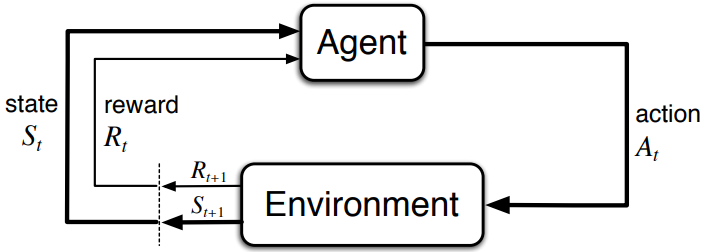
\includegraphics[width=0.6\linewidth]{./chapter3/media/RLConzept}
	\caption[Base concept of Reinforcement Learning]{Base concept of Reinforcement Learning: The Agent interacts with its environment and receives feedback in the form of rewards. Image source:~\cite{sutton2018reinforcement}.}
	\label{fig:RLConzept}
\end{figure}

The agent proceeds in its environment according to the trial-and-error principle to learn this optimal policy. Safety is a critical concern during training, as the agent may execute unpredictable actions while exploring the state space. For this reason, simulation environments are a central component of training and are frequently used for pre-training the policy. The policy is then subsequently often fine-tuned in the real-world environment. Through the trial and error, more efficient, unknown and creative solutions can be found that a human might not have come up with.










% Neuronale Netze

\section{Neural Networks}
Artificial Neural Networks are computational models inspired by the structure and functionality of biological brain and have become a fundamental component of modern machine learning. They are designed to learn complex relationships from data by approximating highly nonlinear functions and are therefore widely used in applications such as image recognition, natural language processing, forecasting and control systems. There exist various types of neural network architectures, including \acfp{CNN} or Transformer models, each tailored to specific types of data and tasks. The following sections provide an overview of the basic functionality of neural networks, their mathematical formulation and the training process.


\subsection{Neuron}
The basic element of an neural network is the neuron. The concept is motivated by biological neurons in the human brain, which communicate through electrochemical signals. In a simplified model, a biological neuron receives signals from other neurons, processes the received information and transmits an output signal~\cite{Lin2017ArtificialNN}. Artificial neurons mimic this behavior mathematically by combining several input values into a single output.

\paragraph{History}
The first mathematical model of an artificial neuron was proposed by McCulloch and Pitts in 1943~\cite{McCulloch1990ALC}. Their model consisted of a binary threshold unit that produced an output only when the weighted sum of its inputs exceeded a predefined threshold and established the foundations for later neural network research.
A major extension of this idea was introduced by Rosenblatt in 1958 with the perceptron~\cite{Rosenblatt1958ThePA}. The perceptron introduced trainable weights to the inputs and a learning rule, making it possible to adapt the model parameters directly from data. However, the perceptron still relied on a threshold-based activation, which produces a linear decision boundary and was therefore limited to linearly separable classification problems~\cite{Minsky1969AnIT}.
This limitation was highlighted by Minsky and Papert, who showed that a single perceptron cannot represent functions such as XOR~\cite{Minsky1969AnIT}. The development of multilayer neural networks together with differentiable activation functions later overcame this restriction. These advances made it possible to train networks with multiple layers and enabled the modern neural network architectures that are used in deep learning today.

\paragraph{Mathematical Formulation}
\begin{figure}[!h]
	\centering
	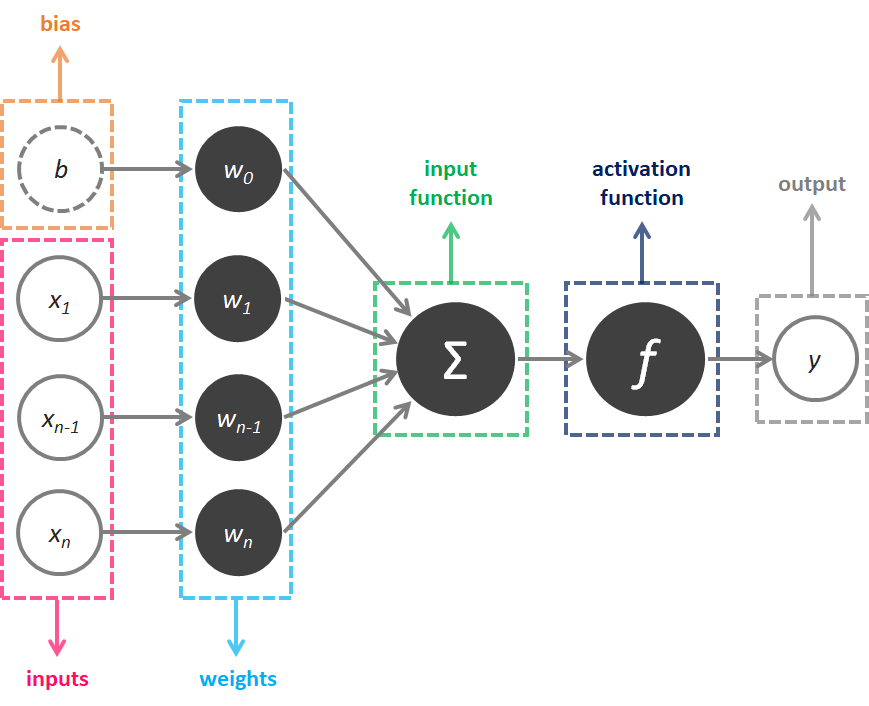
\includegraphics[width=0.55\linewidth]{./chapter2/media/NNNeuron2}
	\caption[Perceptron of an Artificial Neural Network]{Perceptron of an Artificial Neural Network. Image source:~\cite{yseYourGuidePerceptrons2024}.}
	\label{fig:NNIntroModernNeuron}
\end{figure}
A neuron receives an input vector $\mathbf{x}=[x_1,x_2,\ldots,x_n]^T$, where each vector element $x_i$ is associated with a trainable weight $w_i$ from the corresponding weight vector $\mathbf{w} = [w_1, w_2, \ldots, w_n]^T$. The neuron first computes a weighted sum of its inputs and adds a bias term $b$, see \autoref{fig:NNIntroModernNeuron}. The resulting pre-activation value is given by: 
% The weighted inputs are summed together with an optional bias term $(b)$, see \autoref{eq:perceptron}. 
\begin{equation}
    z = \sum_{i=1}^{n} w_i x_i + b
    \label{eq:neuron_scalar}
\end{equation}

The value $z$ represents a linear combination of the input features. To enable the modeling of non-linear relationships, an activation function $\phi(\cdot)$ is subsequently applied, yielding the neuron's output:

\begin{equation}
    y = \phi(z) = \phi\left(\sum_{i=1}^{n} w_i x_i + b\right)
    \label{eq:neuron_activation}
\end{equation}

Without the activation function, a composition of multiple neurons would still correspond to a single linear transformation and therefore could not represent complex non-linear patterns. Common activation functions used in modern neural networks include for example the GeLU, tanh and ReLU.




The weighted sum in \autoref{eq:neuron_scalar} can be expressed more compactly using vector notation and ending in the form of:
\begin{equation}
    y = \phi\!\left(\mathbf{w}^T \mathbf{x} + b\right)
	= \phi\!\left(
        \begin{bmatrix}
            w_1 & w_2 & \cdots & w_n
        \end{bmatrix}
        \begin{bmatrix}
            x_1 \\
            x_2 \\
            \vdots \\
            x_n
        \end{bmatrix}
        + b
    \right) 
    \label{eq:single_neuron}
\end{equation}

This vector formulation serves as the basis for the matrix representation of an entire neural network layer, where multiple neurons are evaluated simultaneously.

\subsection{Neural Networks}
A neural network is a collection of interconnected neurons organized into layers. 
The input layer receives the feature vector, while the output layer produces the final prediction. The hidden layers between the input and output layers perform intermediate computations that allow the network to learn increasingly abstract representations of the input data~\cite{Goodfellow-et-al-2016}.
The parameters of the network (the weights and biases) are learned from data using optimization algorithms such as gradient descent~\cite{Rumelhart1986LearningRB}. As universal function approximators, neural networks are capable of learning complex functions from data, which has made them a powerful tool across numerous applications in machine learning.
% Technically, neural networks are universal function approximators, enabling them to learn complex functions from data and making them a powerful tool for a wide range of applications in machine learning.


To understand the terminology: Artificial neural network is the broadest term, encompassing all brain-inspired, connectionist models. A feedforward neural network is a subcategory where information flows strictly in one direction (from input to output) without forming cycles, but its layers need not be fully connected~\cite{Goodfellow-et-al-2016}. The multilayer perceptron is a feedforward network with one or more fully connected (dense) hidden layers, where every neuron in one layer connects to every neuron in the next~\cite{Goodfellow-et-al-2016}. In a fully connected layer, every neuron is connected to every neuron in the subsequent layer~\cite{Goodfellow-et-al-2016}.
% Each layer consists of multiple neurons and the output of one layer serves as the input to the next layer.

% In general, a neural network consists of multiple interconnected neurons organized into layers
%  and the output of one layer serves as the input to the next layer. 

\paragraph{Multilayer Perceptron Network}
The most common form of such architectures is the \textit{\acf{MLP}}~\cite{Goodfellow-et-al-2016}. In an \ac{MLP}, information flows in one direction from the input layer through one or more fully connected hidden layers to the output layer, where each neuron in a layer receives the outputs of the neurons in the preceding layer as inputs. 
% The output of a layer therefore serves as the input to the next layer.

\begin{figure}[!h]
	\centering
	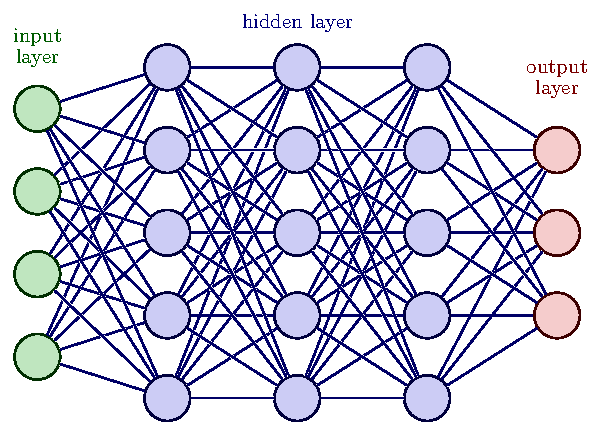
\includegraphics[width=0.55\linewidth]{./chapter2/media/NNNetwork}
	\caption[Neural Networks: Architecture]{Architecture of an Multilayer Perceptron Network. Circles represent perceptrons. Image source:~\cite{NeuralNetworksTikZnet2024}.}
	\label{fig:NNNetwork}
\end{figure}


The computation of an entire layer can be expressed compactly using matrix notation. Let $\mathbf{x}^{(l-1)}$ denote the output vector of the previous layer, $\mathbf{W}^{(l)}$ the weight matrix and $\mathbf{b}^{(l)}$ the bias vector of layer $l$. $M$ are the number of neurons in layer $l$ and $N$ the number of neurons in the previous layer $l-1$. The pre-activation vector is given by:
\begin{equation}
	\mathbf{z}^{(l)} = \mathbf{W}^{(l)} \mathbf{x}^{(l-1)} + \mathbf{b}^{(l)},
\end{equation}
which can be explicitly written as:
\begin{equation}
	\begin{bmatrix}
		w_{11} & \cdots & w_{1N} \\
		w_{21} & \cdots & w_{2N} \\
		\vdots & \ddots & \vdots \\
		w_{M1} & \cdots & w_{MN}
	\end{bmatrix}^{(l)}
	\begin{bmatrix}
		x_1 \\
		x_2 \\
		\vdots \\
		x_N
	\end{bmatrix}^{(l-1)}
	+
	\begin{bmatrix}
		b_1 \\
		b_2 \\
		\vdots \\
		b_M
	\end{bmatrix}^{(l)}
	=
	\begin{bmatrix}
		w_{11}x_1 + \cdots + w_{1N}x_N + b_1 \\
		w_{21}x_1 + \cdots + w_{2N}x_N + b_2 \\
		\vdots \\
		w_{M1}x_1 + \cdots + w_{MN}x_N + b_M
	\end{bmatrix}
\end{equation}

In other words, each neuron in layer $l$ computes its own weighted sum over all outputs of the previous layer and then adds its corresponding bias term. 
Equivalently, the bias can be absorbed into the matrix multiplication by augmenting the input vector with a constant entry $1$ and extending the weight matrix by one additional column:

\begin{equation}
	\begin{bmatrix}
		z_1^{(l)} \\
		z_2^{(l)} \\
		\vdots \\
		z_M^{(l)}
	\end{bmatrix}
	=
	\begin{bmatrix}
		w_{11}^{(l)} & \cdots & w_{1N}^{(l)} & b_1^{(l)} \\
		w_{21}^{(l)} & \cdots & w_{2N}^{(l)} & b_2^{(l)} \\
		\vdots & \ddots & \vdots & \vdots \\
		w_{M1}^{(l)} & \cdots & w_{MN}^{(l)} & b_M^{(l)}
		\end{bmatrix}
		\begin{bmatrix}
		x_1^{(l-1)} \\
		x_2^{(l-1)} \\
		\vdots \\
		x_N^{(l-1)} \\
		1
	\end{bmatrix}
\end{equation}


Then the activation function is applied element-wise to the resulting pre-activation vector $\mathbf{z}^{(l)}$ to produce the output of layer $l$:
\begin{equation}
	\mathbf{x}^{(l)} = \phi(\mathbf{z}^{(l)}) = \phi\!\left(\mathbf{W}^{(l)} \mathbf{x}^{(l-1)} + \mathbf{b}^{(l)}\right).
\end{equation}



\paragraph{Non-Linear Activation Functions in Neural Networks}
The introduction of non-linear activation functions is essential, as a composition of purely linear transformations would again result in a linear model~\cite{Goodfellow-et-al-2016}. By combining multiple layers with non-linear activations, neural networks can approximate highly complex functions and learn non-linear, intricate patterns from data~\cite{Hornik1991ApproximationCO}. 
% In fact, sufficiently large neural networks are universal function approximators, meaning they can approximate a wide range of continuous functions to arbitrary accuracy. 
Common activation functions used in modern neural networks include the functions GELU~\cite{Hendrycks2016GaussianEL}, ReLU~\cite{Nair2010RectifiedLU}, Leaky ReLU~\cite{Maas2013RectifierNI}, the tanh~\cite{Ryck2021OnTA} and the Swish function~\cite{Ramachandran2017SwishAS}. But there exist many more. Each of these functions has its own characteristics and can result in different learning dynamics and performance. 





\paragraph{Prediction}
The output layer produces the network's final prediction, and the choice of its activation function is crucial, as it determines how predictions are interpreted and which loss function is used during training:
% The output layer is responsible for producing the network's final prediction. Its activation function is chosen based on the task: 
\begin{itemize}
	\item \textbf{Regression:} A linear activation directly outputs a continuous value.
	\item \textbf{Binary Classification:} A single neuron with a sigmoid function outputs a probability between 0 and 1.
	\item \textbf{Multi-Class Classification:} A softmax layer produces a probability distribution over the classes, where each output neuron corresponds to a specific class and the softmax function ensures that the outputs sum to 1, representing the predicted probabilities for each class.
\end{itemize}
% The choice of activation function in the output layer is crucial, as it directly affects the interpretation of the network's predictions and the appropriate loss function to use during training.




\paragraph{Loss Function}
The loss function $\mathcal{L}$ is a measure of how well the network is able to predict the target value and quantifies the difference between the network's predictions and the true labels in the training data. The goal of the training process is to minimize the loss function by adjusting the weights of the network. The loss function can be any differentiable function, but common choices are \acf{MSE} for regression tasks and cross-entropy for classification tasks.
\begin{itemize}
	\item \textbf{\acf{MSE} Loss Function:} Commonly used for regression tasks, where the goal is to predict continuous values and is defined as:
	\begin{equation}
		\mathcal{L} = \frac{1}{N} \sum_{i=1}^{N} (y_i - \hat{y}_i)^2
	\end{equation}
	where $y_i$ is the target value for the $i$-th sample, $\hat{y}_i$ is the predicted value for the $i$-th sample and $N$ is the number of samples.
	

	\item \textbf{Cross-Entropy Loss Function:} Commonly used for classification tasks, where the goal is to predict discrete class labels. 
	For binary classification problems, the network typically uses a single output neuron with a sigmoid activation. The output $\hat{y}_i \in [0,1]$ represents the predicted probability of the positive class. The binary cross-entropy loss is then defined as:
		\begin{equation}
			\mathcal{L} =
			-\frac{1}{N}\sum_{i=1}^{N}
			\left(
			y_i \log(\hat{y}_i) + (1 - y_i)\log(1 - \hat{y}_i)
			\right)
		\end{equation}
		where $y_i \in \{0,1\}$ denotes the true label of the $i$-th sample, $\hat{y}_i$ is the predicted probability of the positive class and $N$ is the number of samples.

		For multi-class classification problems with $C$ classes, the network output is typically normalized using a softmax function to obtain a probability distribution over all classes (which sums up to 1 over the classes). The corresponding cross-entropy loss is defined as:
		\begin{equation}
			\mathcal{L} =
			-\frac{1}{N}\sum_{n=1}^{N}\sum_{i=1}^{C}
			y_{n,i}\log(\hat{y}_{n,i})
		\end{equation}
		where $y_{n,i}$ represents the one-hot encoded ground-truth label and $\hat{y}_{n,i}$ is the predicted probability for class $i$ of sample $n$.

\end{itemize}
















\subsection{Training Neural Networks}
% gradient based optimization
The parameters of a neural network, namely the weights and biases, are learned from data during training. This is typically achieved by minimizing a loss function $\mathcal{L}$ using optimization methods such as gradient descent and its variants. The gradients required for optimization are efficiently computed using the backpropagation algorithm, which propagates the prediction error from the output layer back through the network~\cite{Rumelhart1986LearningRB}. This learning process enables neural networks to adapt their weights and achieve strong performance across a wide range of machine learning tasks.

\paragraph{What is a Gradient?} 
The gradient describes how a function changes with respect to its input variables and points in the direction of the steepest increase of the function~\cite{Rumelhart1986LearningRB, Bottou2016OptimizationMF}. In the special case of a function with only one variable, the gradient reduces to the first derivative, which corresponds to the slope of the function at a given point.
In simple terms, the gradient indicates how the function value changes when making a small step to the right or left away from a specific point.



% In Figure~\ref{fig:NNGradientIntro}, the gradient is represented by the slope of the curve at a particular point. It indicates how the function value changes when moving slightly away from that point.
% The gradient is represented by the slope of the curve at a particular point. 
To better understand the concept of gradients, consider \autoref{fig:NNGradientIntro}. The Goal is to determine the slope of the blue curve at $x=1$. For the function $f(x)=x^2-3$, the derivative is $f'(x)=2x$, which is evaluated at $x=1$. $f'(1)=2$ and means the slope of the curve at this point is 2. To verify this result, the slope triangle is shown in \autoref{fig:NNGradientIntro}. It provides a visual representation of the slope and confirms the calculated value of with the slope $m=2$.
In general, the gradient indicates whether a function is increasing or decreasing at a specific point and how steeply it changes. A positive gradient means that the function is increasing, while a negative gradient indicates that the function is decreasing. The magnitude of the gradient describes how steeply the function changes. Larger magnitudes correspond to steeper slopes, while values close to zero indicate relatively flat regions.

\begin{figure}[!h]
	\centering
	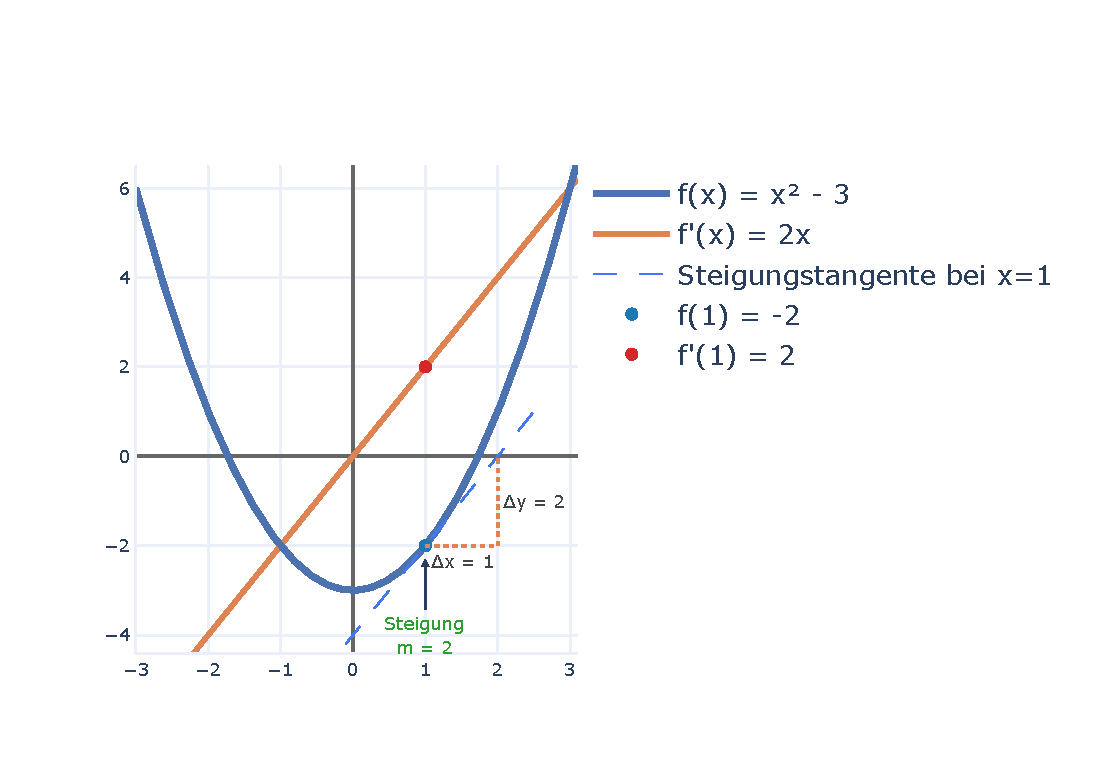
\includegraphics[width=0.85\linewidth]{./chapter2/media/NNGradientIntro.pdf}
	\caption[Understanding Gradients]{Understanding Gradients: The gradient of a 1D function $f(x)$ at point $x=1$ is calculated with the derivative $f'(x)$. It represents the slope of the tangent line at that point.}
	\label{fig:NNGradientIntro}
\end{figure}





\paragraph{Gradient Descent and Parameter Update} 
Gradient descent is an iterative optimization algorithm that is used to minimize a loss function~\cite{Bottou2016OptimizationMF}.
The basic principle of gradient descent can be understood by considering a simplified setting with a single parameter, which illustrates a network weight, see \autoref{fig:NNGradientDescent_2}. 
The horizontal axis represents the value of the weight, while the vertical axis represents the corresponding loss, which quantifies the discrepancy between the predicted and true values of the training data.

\begin{figure}[!h]
	\centering
	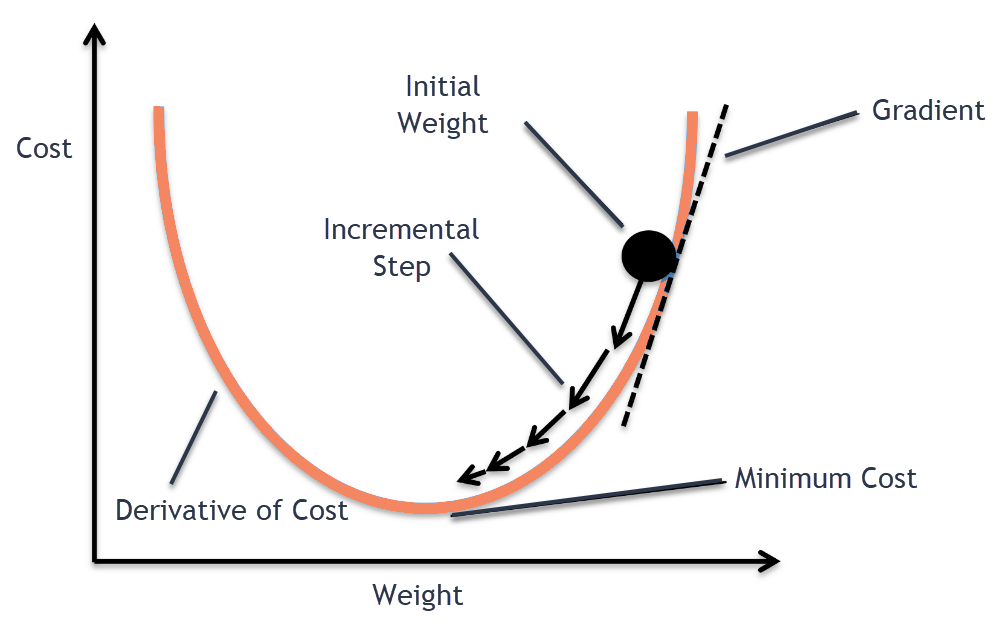
\includegraphics[width=0.6\linewidth]{./chapter2/media/NNGradientDescent_2}
	\caption[Neural Network: Simplified Gradient Descent]{Simplified gradient descent based on one network weight. Image source:~\cite{lanhamLearnARCoreFundamentals}.}
	\label{fig:NNGradientDescent_2}
\end{figure}

The resulting curve is the loss landscape for that one parameter. 
% At any point on the loss curve, the derivative (or gradient) indicates the local slope of the function.
% The current network weight, shown by the black dot must be updated in a way, to reduce the loss.
The current value of the weight, represented by the black dot, must be adjusted such that the loss decreases. Gradient descent achieves this through the following two steps:
\begin{enumerate}
	\item \textbf{Calculate the gradient:} 
	Compute the gradient of the loss function with respect to the weight. 
	% The gradient of the loss function with respect to the weight is calculated.
	% The first step is to compute the gradient of the loss function with respect to the weight. 
	The gradient indicates how the loss changes as the weight is adjusted.
	% The gradient of the loss function with respect to the parameter is calculated.
	\item \textbf{Update the weight:} The weight is then updated by moving in the opposite direction of the gradient. 
	Since the gradient points towards the direction of steepest increase, moving against it results in a reduction of the loss.
	% This is because the gradient points in the direction of steepest ascent, so moving in the opposite direction will lead to a decrease in the loss. 
	The basic parameter update is defined as:
	\begin{equation}	
		\mathbf{W}_{\text{t+1}} = \mathbf{W}_{\text{t}} - \alpha \cdot \nabla \mathcal{L}(\mathbf{W}_{\text{t}})
	\end{equation}
	where $\alpha$ denotes the learning rate, which controls the step size of the update and $\nabla \mathcal{L}(\mathbf{W}_{\text{t}})$ is the gradient of the loss function with respect to the parameter at iteration $t$.
	% where $\alpha$ is the learning rate, a hyperparameter that controls the step size of the update and $\nabla L(W_{\text{t}})$ is the gradient of the loss function with respect to the weight at its current value.	
\end{enumerate}


% In the example shown in Figure 2.5, the gradient is positive. Consequently, increasing the weight would increase the loss. To reduce the loss, the weight must therefore be moved in the opposite direction (to the left).
In the example shown in \autoref{fig:NNGradientDescent_2}, the gradient is positive. To reduce the loss, the weight must therefore be moved to the left, to the highest decrease of the function which is the negative gradient.
%  in the opposite direction (to the left). 
This procedure is repeated iteratively until the algorithm reaches a minimum of the loss function or another stopping criterion is satisfied. The successive parameter updates are illustrated by the black arrows in \autoref{fig:NNGradientDescent_2}. At the minimum, the gradient/the slope are zero and the parameter update becomes zero as well. The algorithm has converged. 
The goal is to find the optimal set of parameters that minimizes the loss function, which corresponds to the best fit of the model to the data, meaning the network's predictions are sufficiently accurate~\cite{Bottou2016OptimizationMF}. 




\paragraph{Optimization Problems}
Not every minimum found is a good solution. The loss landscape of neural networks is highly non-convex and can contain many local minima, saddle points and flat regions, where the gradient is zero but the loss is not minimized. If the gradient gets zero, the optimization process get stuck~\cite{Bottou2016OptimizationMF}. \autoref{fig:NNNetwork_OptimizationProblems} shows a loss landscape with two parameters. The black dot represents the inital parameter values and the line shows the trajectory of the parameter updates during training. As seen it depends on the initial parameter values, whether the algorithm converges to the global minima, local minama or to the saddle point in the middle of the two hills.  


\begin{figure}[!h]
	\centering
	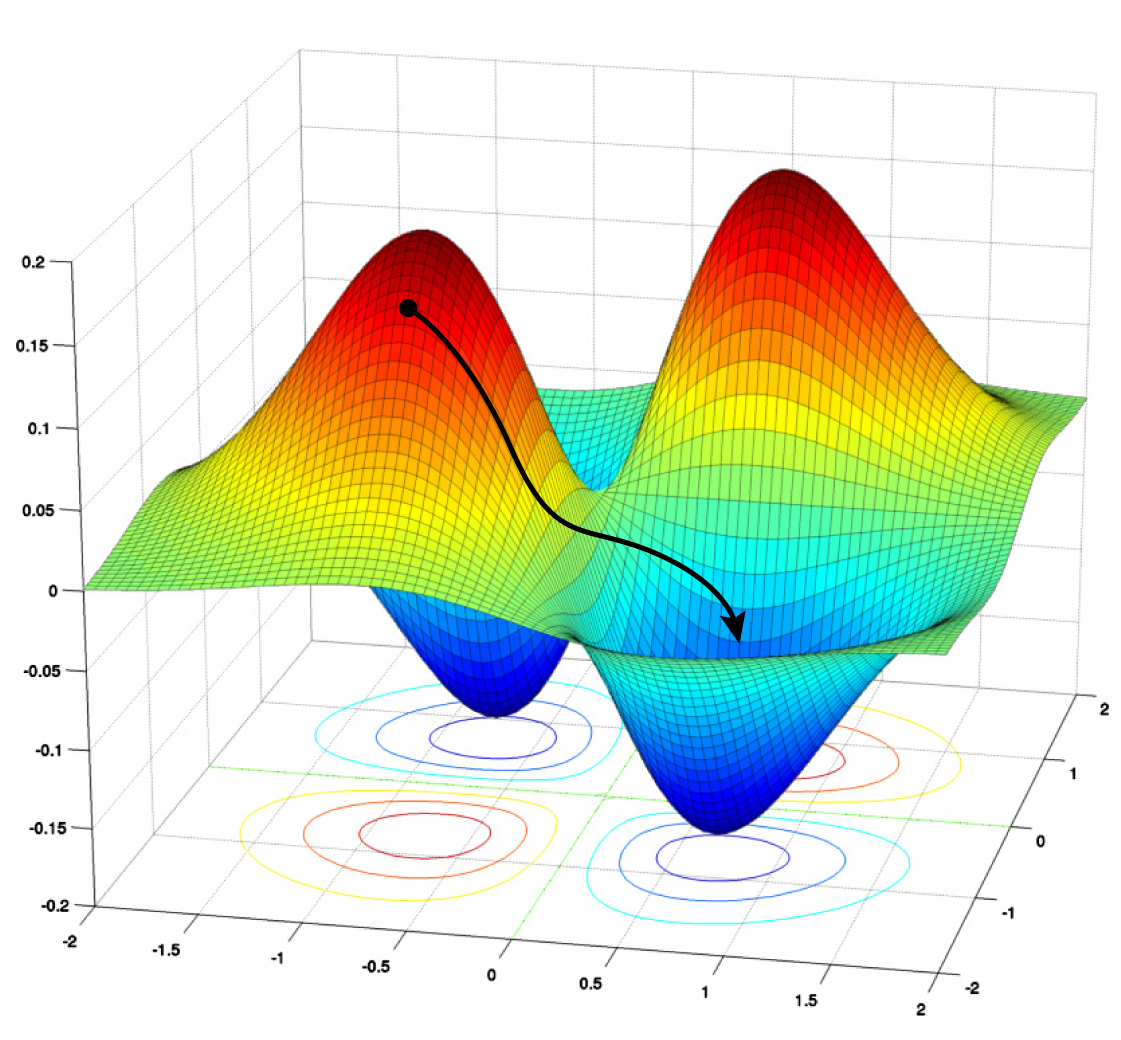
\includegraphics[width=0.5\linewidth]{./chapter2/media/NNGradientDescent}
	\caption[Neural Networks: Optimization Problems]{Neural Networks and their optimization Problems: The figure shows a loss landscape of two parameters, which has a local minima and a saddle point, where the training precess could get stuck. Image source:~\cite{ananthaswamyResearchersBuildAI2022}.}
	\label{fig:NNNetwork_OptimizationProblems}
\end{figure}

In the shown examples, the loss landscape was known, but in practice, the loss landscape of neural networks is typically unknown and can be highly complex.  Neural networks often consists of millions of parameters and therefore they have a high-dimensional loss landscape. The Algorithm works in such high-dimensional spaces in the same way.
% The optimization process works in such high-dimensional spaces in the same way and navigates through this loss landscape to find a set of parameters that minimizes the loss function. 
Therefore, training neural networks can be challenging and may require careful tuning of hyperparameters such as the learning rate, as well as the use of techniques like momentum, adaptive learning rates or regularization to improve convergence and generalization performance~\cite{Bottou2016OptimizationMF}. For this many variants of the basic gradient descent algorithm have been developed.


% \textit{Backpropagation.}
% The gradients needed for the parameter updates in gradient descent are computed using the backpropagation algorithm. Backpropagation efficiently propagates the error from the output layer back through the network to compute the necessary gradients for all parameters. For each neuron, the corresponding proportion of the total error is calculated and the weights are adjusted accordingly. 

\paragraph{Backpropagation}
The gradients required for updating the network parameters are computed using the backpropagation algorithm~\cite{Rumelhart1986LearningRB}. Backpropagation efficiently propagates the prediction error from the output layer back through the network and computes the gradients of the loss function $\mathcal{L}$ with respect to all weights $\mathbf{W}$ in the model. Based on these gradients, each parameter $w_{ij}^l$ is adjusted proportionally to its contribution to the overall error.
More precisely, backpropagation computes the partial derivatives of the loss function with respect to all trainable parameters in the network. These gradients quantify how sensitive the loss is to small changes in each parameter and therefore indicate how each parameter should be adjusted to reduce the overall error. Parameters that contribute more strongly to the error receive larger updates, while less influential parameters are adjusted more mildly.
The training process for a neural network can therefore be summarized by the following update rule:
\begin{equation}
\mathbf{W}_{t+1} = \mathbf{W}_t - \alpha \cdot \nabla_{\mathbf{W}_t} \left( \frac{1}{N} \sum_{i=1}^{N} \mathcal{L}\bigl(\mathbf{y}_i, f_{\mathbf{W}_t}(\mathbf{x}_i)\bigr) \right)
\end{equation}
where $f_{\mathbf{W}}$ denotes the neural network with parameters $\mathbf{W}$, $\mathcal{L}$ is the loss function measuring the difference between the predicted output $f_{\mathbf{W}}(\mathbf{x}_i)$ and the target value $\mathbf{y}_i$, $\alpha$ is the learning rate, $N$ is the number of training samples and $\nabla_{\mathbf{W}_t}$ represents the gradient of the loss function with respect to the weights at iteration $t$.
By iteratively applying this update rule, the network parameters are gradually adjusted in a direction that reduces the loss function and allows neural networks to reduce improve their predictions from training data.
% learn meaningful representations from training data
% . This iterative optimization process is what allows the neural network to learn meaningful representations from training data and improve its predictions over time.


Besides the standard gradient descent algorithm, which computes the gradient over the entire dataset, several more efficient variants are commonly used in practice. 
Instead of computing the gradient on the entire dataset, the variants stochastic and mini-batch gradient descent approximate it using one or a few training samples~\cite{Bottou2010LargeScaleML, Robbins1951ASA, Bottou2016OptimizationMF, Goodfellow-et-al-2016}, which reduces the computational cost per update while still providing a more stable gradient estimate compared to pure stochastic gradient descent.





\paragraph{Evaluation}
To measure the performance of a machine learning model, various evaluation metrics can be used depending on the specific task and problem setting. These metrics provide quantitative measures of how well a model performs and allow comparisons between different models or configurations. While common examples include accuracy, precision, recall and the F1-score for classification tasks, as well as mean squared error for regression tasks. However, a detailed discussion of these metrics is beyond the scope of this work.

The performance of a machine learning model is typically evaluated using data that has not been seen during training, referred to as test data. This allows an unbiased assessment of the model's ability to generalize to new, unseen samples. There exist in general three main scenarios regarding the model's performance on training and test data:
\begin{itemize}
	\item \textbf{Underfitting:} A model that underfits performs poorly on both training and test data. It fails to capture the underlying patterns in the training data, resulting in high error on both datasets.
	\item \textbf{Overfitting:} An overfitted model achieves high performance on the training data but fails to generalize well to the test data. It has essentially memorized the training samples, including noise and outliers, which leads to poor performance on new data.
	\item \textbf{Well-Balanced Model:} A well-balanced model achieves consistently good performance on both training and test datasets. It captures the underlying patterns in the training data without overfitting, allowing it to generalize effectively to unseen samples. 
\end{itemize}






\section{Convolutional Neural Networks}

A Convolutional Neural Network (CNN) is a deep neural network architecture designed to process grid-like data, especially images~\cite{LeCun1998GradientbasedLA, Krizhevsky2012ImageNetCW}. CNNs are particularly effective for visual tasks because they exploit the spatial structure of an image and learn local patterns such as edges, corners and textures. Unlike fully connected networks, CNNs do not treat every pixel independently. Instead, they use small learnable filters that are applied across the image to detect relevant structures at different positions~\cite{Khan2025ACS, Younesi2024ACS, Long2022}.

\paragraph{Convolution}

The main idea of a CNN is the convolution operation, where a filter, also known as kernel, is applied to the image to extract features. For example, the Prewitt kernels, also known as edge detection filters, can be used to detect horizontal and vertical edges in an image:
\begin{equation}
	K_{\text{horizontal}} =
	\begin{bmatrix}
		-1 & 0 & 1\\
		-1 & 0 & 1\\
		-1 & 0 & 1
	\end{bmatrix}
	\qquad
	K_{\text{vertical}} =
	\begin{bmatrix}
		-1 & -1 & -1\\
		0 & 0 & 0\\
		1 & 1 & 1
	\end{bmatrix}
\end{equation}

\autoref{fig:CNNCatPrewitt} shows the result, after applying the Prewitt kernels to a grey-scale image. There exists a wide variety of predefined filters to extract various of visual structures from the image. 
\begin{figure}[h]
    \centering
    \subfigure[Original Image: No convolution is applied]{
        \parbox{4.6cm}{
            \centering
            {\small\textbf{Original}}\par
            \vspace{0.3em}
            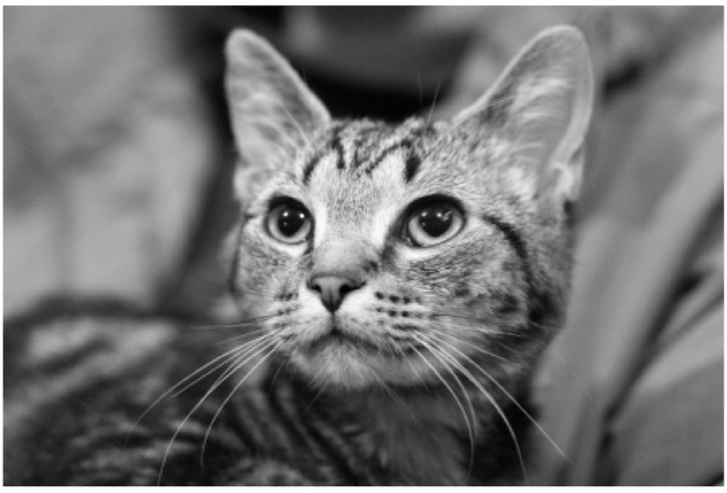
\includegraphics[width=4.5cm]{./chapter2/media/CNNCatPrewittOriginal_3}
        }
        \label{fig:CNNCatPrewittOriginal}
    }
    \hspace{0.3cm}
    \subfigure[Convolved Image, after the horizontal Prewitt kernel is applied to the original image]{
        \parbox{4.7cm}{
            \centering
            {\small\textbf{Horizontal Prewitt}}\par
            \vspace{0.3em}
            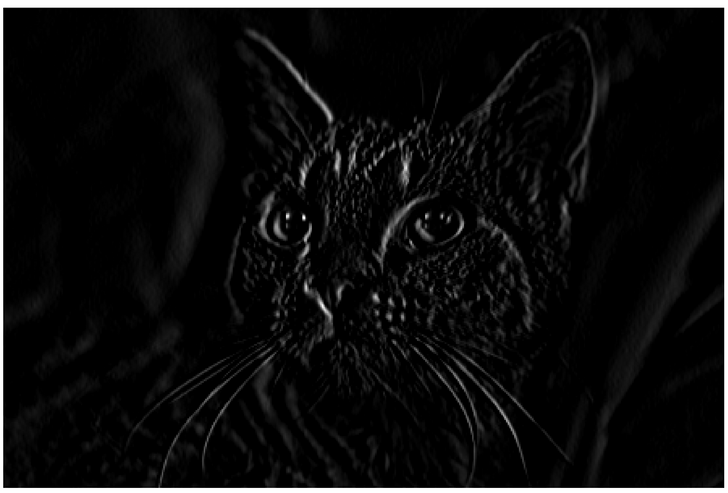
\includegraphics[width=4.5cm]{./chapter2/media/CNNCatPrewittHorizontal_3}
        }
        \label{fig:CNNCatPrewittHorizontal}
    }
    \hspace{0.3cm}
    \subfigure[Convolved Image, after the vertical Prewitt kernel is applied to the original image]{
        \parbox{4.6cm}{
            \centering
            {\small\textbf{Vertical Prewitt}}\par
            \vspace{0.3em}
            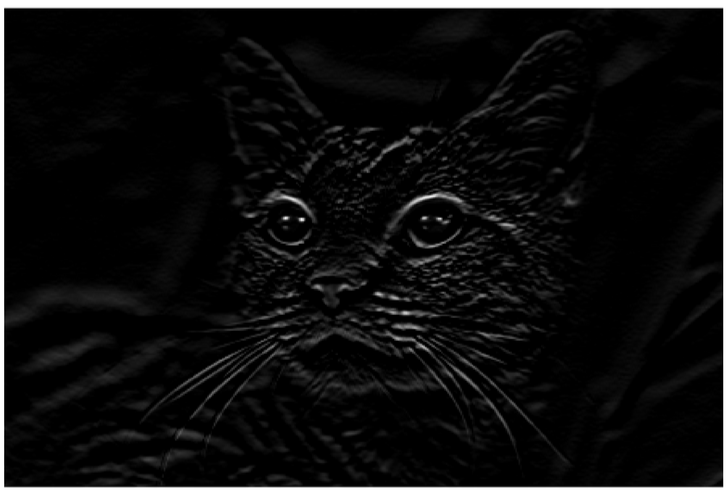
\includegraphics[width=4.5cm]{./chapter2/media/CNNCatPrewittVertical_3}
        }
        \label{fig:CNNCatPrewittVertical}
    }
    \caption[CNN: Convolution of a Greyscale Image using Prewitt Kernels]{Convolution of a greyscale image using Prewitt kernels. Image sources:~\cite{UnderstandingFiltersConvolutional}.}
    \label{fig:CNNCatPrewitt}
\end{figure}




A Filter or kernel is defined as a small matrix of weights, is moved across the image and element-wise multiplied with the underlying pixel values~\cite{Dumoulin2016AGT, Khan2025ACS, Younesi2024ACS, Long2022}. This is possible, because an image is technically a matrix of pixel values too. The resulting values are stored in a new matrix called a feature map, which highlights the patterns detected by the kernel. Since the same kernel is reused at every pixel location, CNNs are able to detect the same feature independent of its position in the image.
% Figure \autoref{fig:CNNConvolutionIntro} illustrates the mathematical convolution operation, where a $3 \times 3$ kernel is applied to a $6 \times 6$ image. The results are stored in a $3 \times 3$ matrix. 

During the convolution process, a kernel (dark blue) slides across the image (light blue), and at each position the element-wise products are summed to generate a single output value that is stored in the feature map (olive green), as shown in \autoref{fig:CNNConvolution_1}.
Figure~\ref{fig:CNNConvolutionIntro} illustrates the mathematical convolution operation, where a $3 \times 3$ kernel is applied to a $6 \times 6$ image to produce a $3 \times 3$ output matrix. 
\begin{figure}[!h]
	\centering
	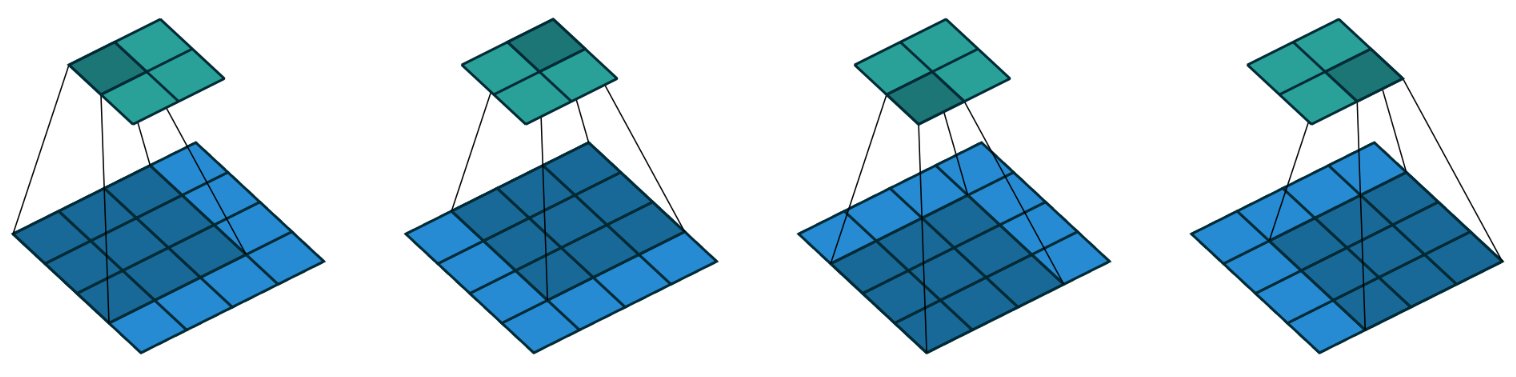
\includegraphics[width=0.75\linewidth]{./chapter2/media/CNNConvolution_1.png}
	\caption[CNN Convolution: Convolution of an Image with the Resulting Feature Map]{Convolution of an image with the resulting feature map. Image source:~\cite{Dumoulin2016AGT}.}
	\label{fig:CNNConvolution_1}
\end{figure}

\begin{figure}[!h]
	\centering
	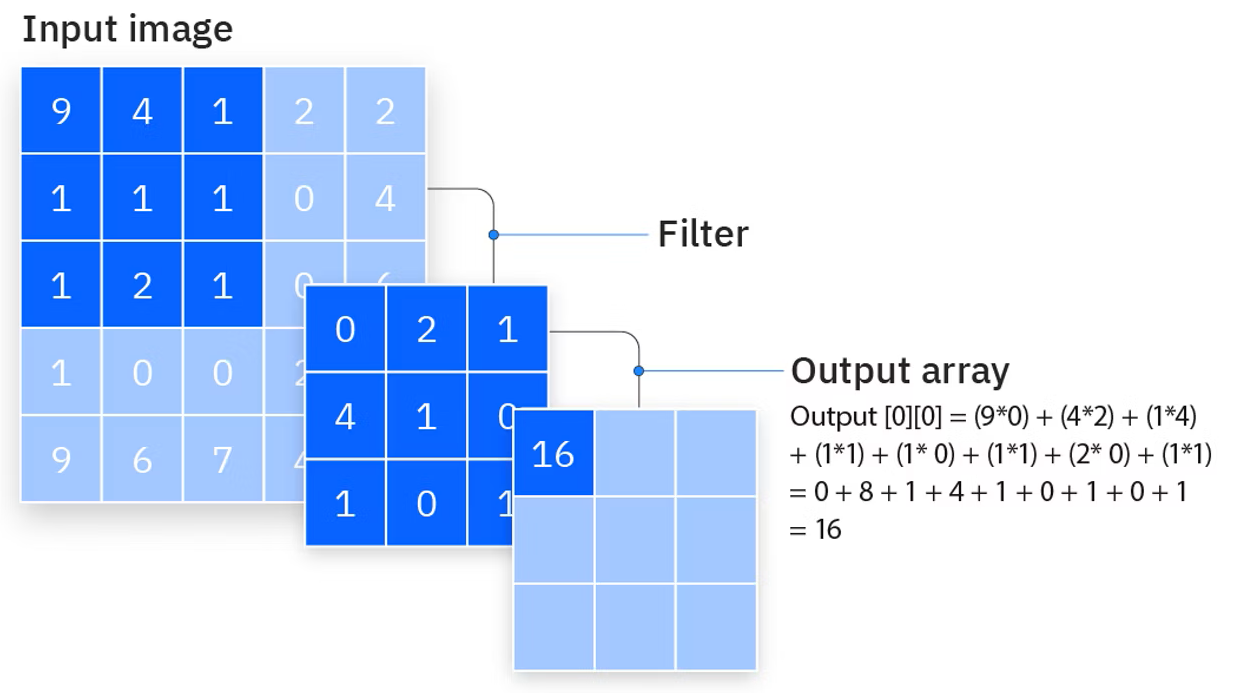
\includegraphics[width=0.65\linewidth]{./chapter2/media/CNNConvolutionIntro.png}
	\caption[CNN Convolution: Mathematical concept]{Mathematical concept of the convolution in \acsp{CNN} using element-wise multiplication. Image source:~\cite{WhatAreConvolutional2021}.}
	\label{fig:CNNConvolutionIntro}
\end{figure}

% Figure \autoref{fig:CNNConvolution_1} shows how the kernel (dark blue) is slided across the image (light blue) step by step. At each location the element-wise products are summed up to obtain one output value, which is stored in a feature map (olive green). 

A CNN consist of multiple kernels, which are applied in parallel and in multiple layers to the image, resulting in multiple feature maps. Importantly, in a CNN the kernels are not fixed manually, instead they are learned during training, allowing the network to find the optimal filters for the task success~\cite{Khan2025ACS, Younesi2024ACS, Long2022}.


% Figures \autoref{fig:CNNConvolutionIntro_View2} shows an alternative view of the convolution process.
% \begin{figure}[!h]
% 	\centering
% 	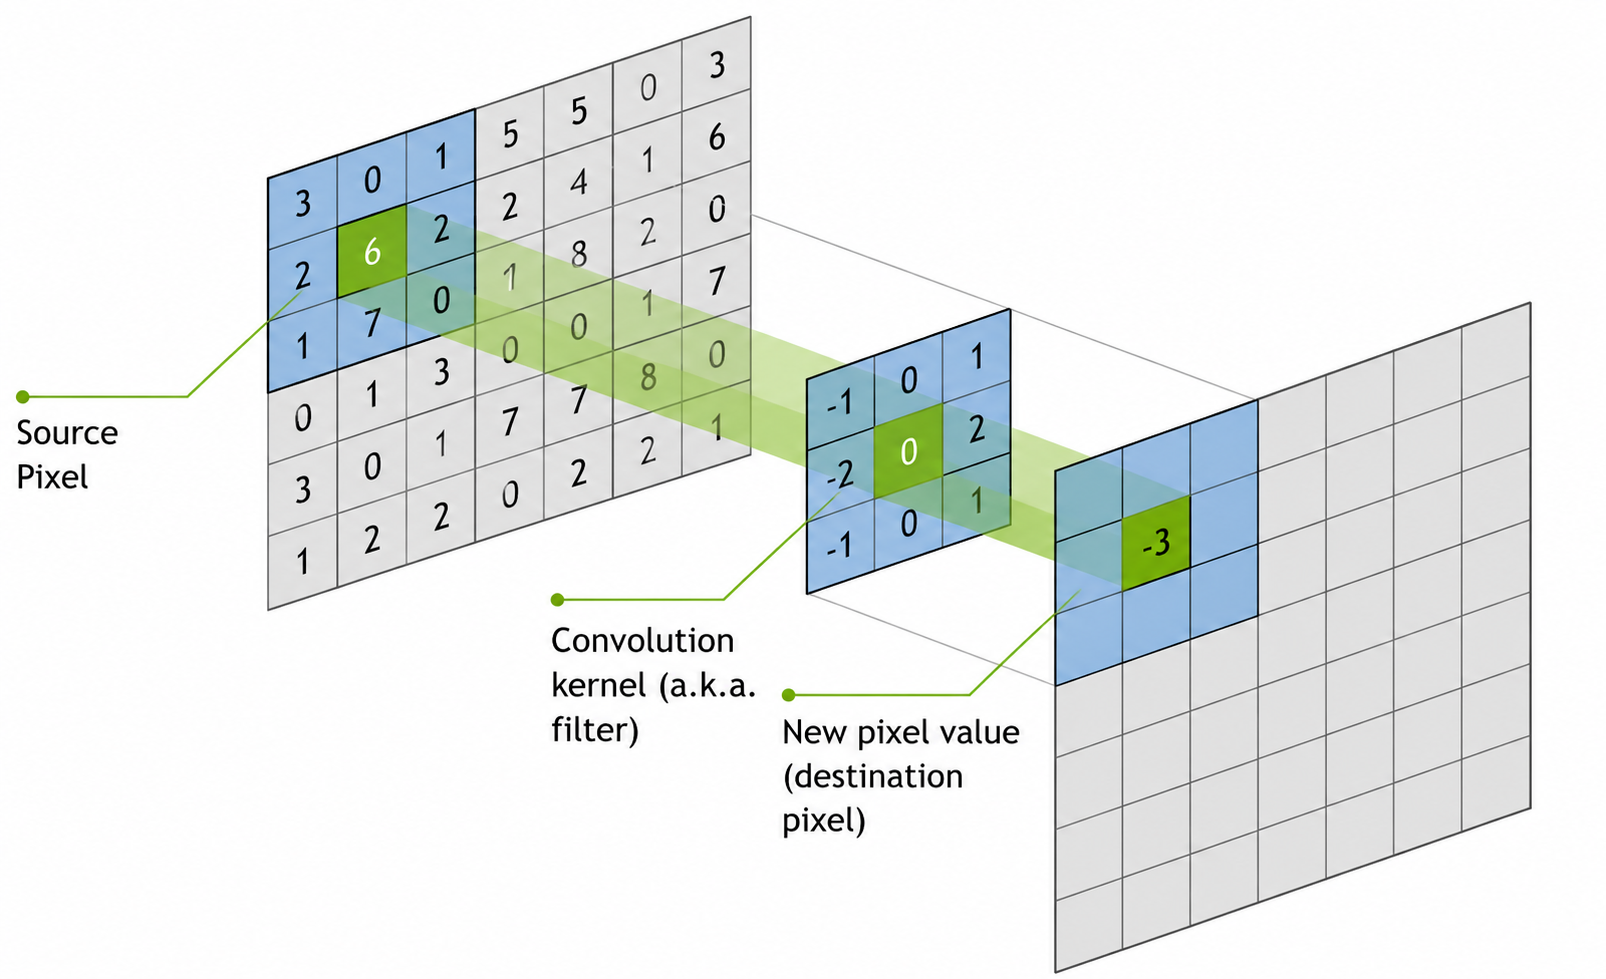
\includegraphics[width=0.65\linewidth]{./chapter2/media/CNNConvolutionIntro_View2.png}
% 	\caption[CNN Convolution Introduction]{CNN Convolution Introduction. Image adapted from:~\cite{WhatConvolutionalNeural}.}
% 	\label{fig:CNNConvolutionIntro_View2}
% \end{figure}


\paragraph{Padding}
As seen in the Figures \ref{fig:CNNConvolutionIntro} and \ref{fig:CNNConvolution_1}, the feature map is smaller than the original image, because of the convolution operation. 
To preserve the spatial resolution of the input image, padding is often added around the border before applying the convolution, see \autoref{fig:CNNConvolution_1_withPadding}~\cite{Dumoulin2016AGT, Khan2025ACS, Younesi2024ACS, Long2022}. With zero-padding, the image size can remain unchanged after the convolution, which is useful when multiple convolution layers are stacked. 
\begin{figure}[!h]
	\centering
	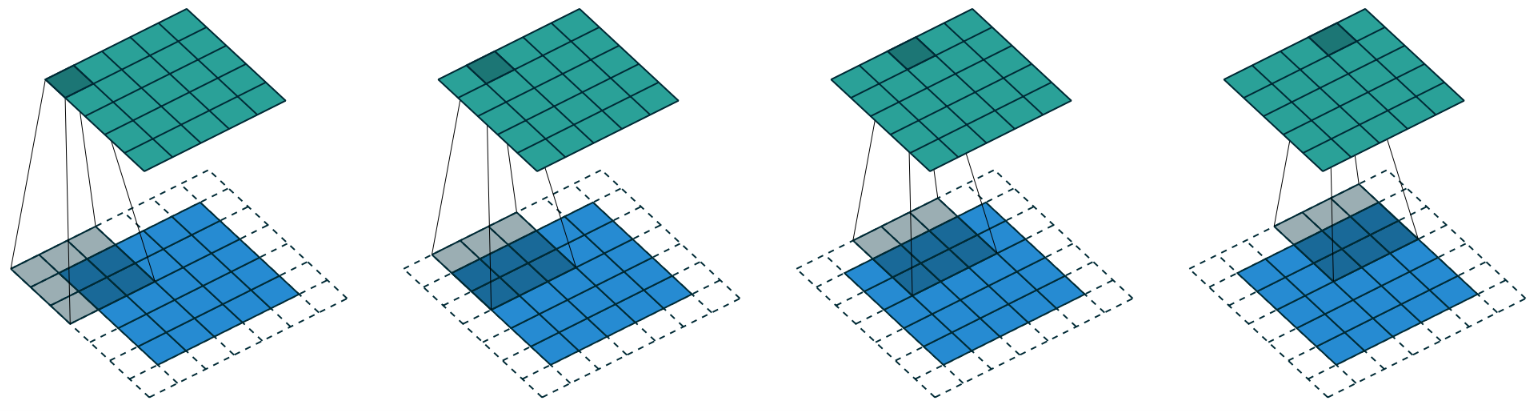
\includegraphics[width=0.75\linewidth]{./chapter2/media/CNNConvolution_1_withPadding}
	\caption[CNN Convolution with Padding]{CNN Convolution with Padding. Image source:~\cite{Dumoulin2016AGT}.}
	\label{fig:CNNConvolution_1_withPadding}
\end{figure}





\paragraph{Activation Function}
After the convolution operation, a non-linear activation function is applied to the resulting feature map~\cite{Khan2025ACS, Younesi2024ACS, Long2022}. Activation functions introduce non-linearity into the network, allowing CNNs to learn complex visual patterns that cannot be represented by linear transformations alone~\cite{Hanin2017ApproximatingCF}.
The most commonly used activation function is ReLU~\cite{Khan2025ACS, Hanin2017ApproximatingCF, Long2022}:
which replaces all negative values with zero while leaving positive values unchanged:
\begin{equation}
	f(x)=\max(0,x)
\end{equation}
By applying the ReLU function after each convolution, the network can learn increasingly complex feature representations across multiple layers.


\paragraph{Pooling Layer}
Another central component of CNNs is the pooling layer~\cite{Khan2025ACS, Long2022}. Pooling reduces the spatial size of the feature maps while retaining the most important information. This lowers the computational cost and increases robustness to small shifts in the input image.
A common choice is a $2\times2$ pooling window with a stride of 2. In this case, the feature map is divided into non-overlapping $2\times2$ regions and each region is summarized by a single value~\cite{Younesi2024ACS, Khan2025ACS}. As a result, the width and height of the feature map are reduced by a factor of two.

Two common pooling methods are max pooling and average pooling~\cite{Younesi2024ACS, Khan2025ACS}, as illustrated in \autoref{fig:CNNPooling}. In max pooling, the largest value within each pooling region is selected and propagated to the output feature map. In average pooling, the mean value of all elements within the region is computed. Both methods reduce the spatial resolution while preserving the most relevant information contained in the feature map.
Pooling layers are typically applied after convolution layers and allow the network to build increasingly compact feature representations. While early convolution layers extract local patterns such as edges and textures, pooling helps summarize these features and enables deeper layers to focus on higher-level visual structures~\cite{Younesi2024ACS, Khan2025ACS, Long2022}.

\begin{figure}[!h]
	\centering
	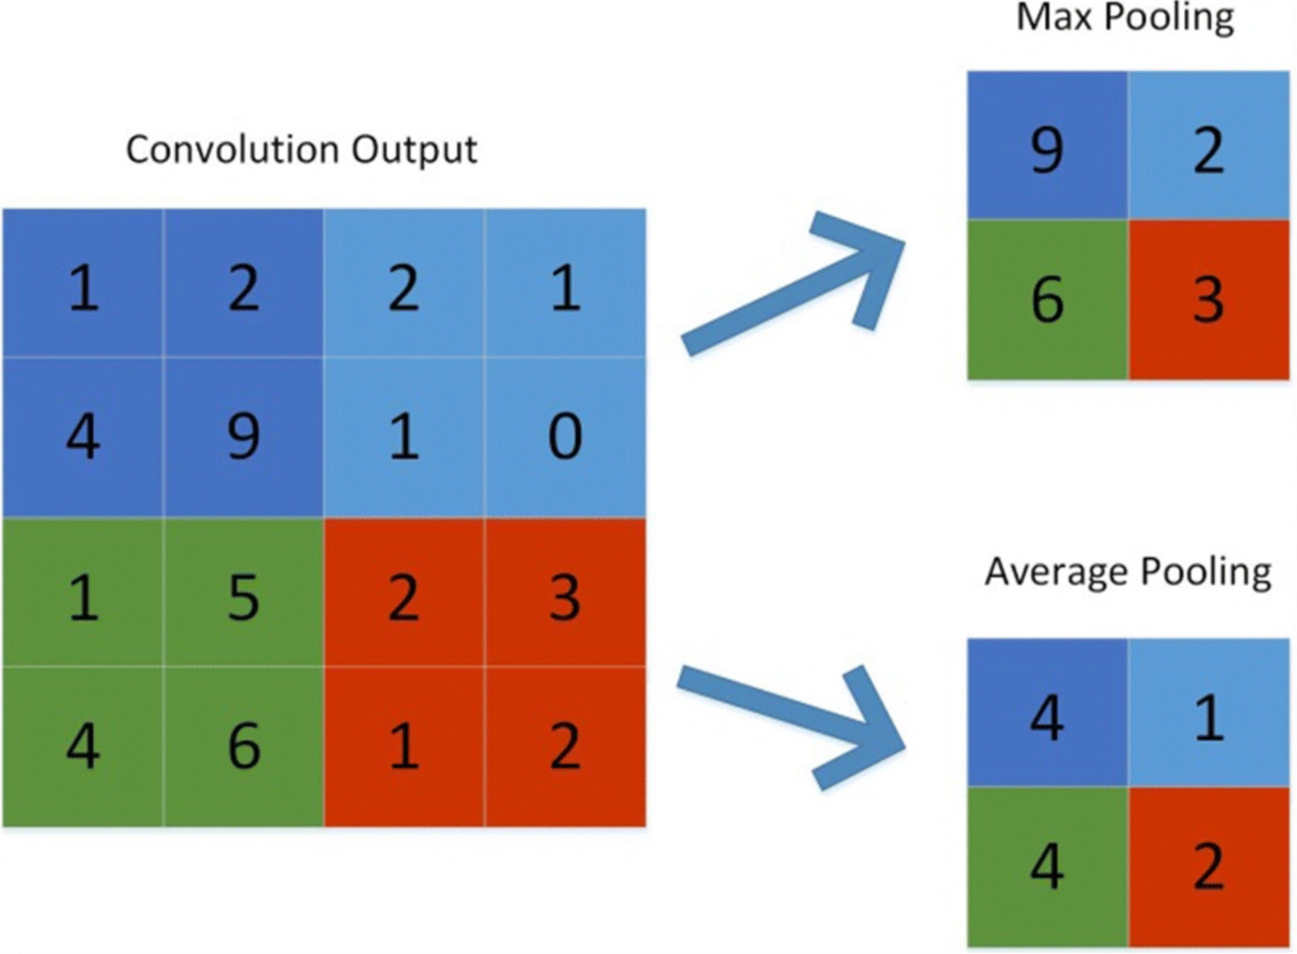
\includegraphics[width=0.4\linewidth]{./chapter2/media/CNNPooling}
	\caption[CNN Pooling]{CNN Pooling: Illustration of max pooling and average pooling operations with a stride of 2. Image source:~\cite{jiangEightlayerConvolutionalNeural2020}.}
	\label{fig:CNNPooling}
\end{figure}
% \begin{figure}[!h]
% 	\centering
% 	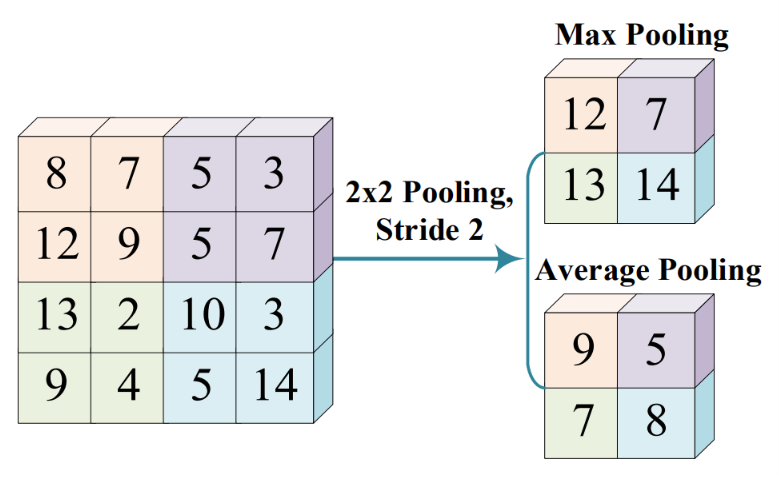
\includegraphics[width=0.45\linewidth]{./chapter2/media/CNNPooling_2.png}
% 	\caption[CNN Pooling]{CNN Pooling. Image source:~\cite{Khan2025ACS}.}
% 	\label{fig:CNNPooling}
% \end{figure}


\paragraph{CNN Pipeline}

The common CNN processing sequence is: convolution, activation function and pooling, while the activation function is often not mentioned explicitly.
A CNN usually consists of several repeated blocks of convolution and pooling layers. Early layers detect simple features such as edges and corners, while deeper layers combine these basic features into more complex structures. 
After several convolution and pooling stages, the feature maps are flattened into one big vector and passed through a MLP or a classification head in a classification task to produce the final predictions, see \autoref{fig:CNNPipeline}. Through backprobagating the prediction error, the networks parameter are adjusted during training.

\begin{figure}
	\centering
	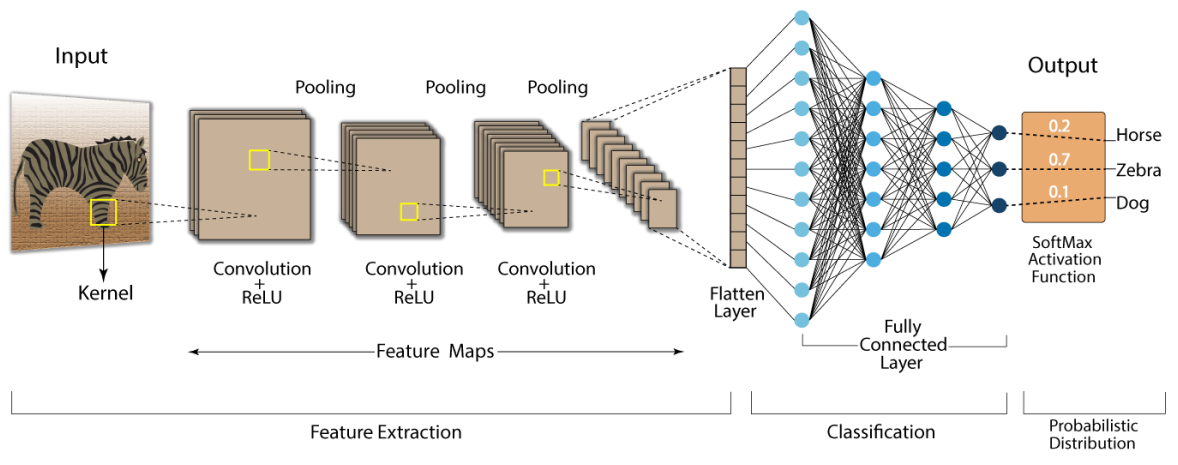
\includegraphics[width=1.0\linewidth]{./chapter2/media/CNNPipeline.png}
	\caption[CNN Pipeline]{CNN Pipeline: Illustration of the typical processing sequence in a CNN, including convolution, activation function, and pooling layers. Image source:~\cite{swapnaConvolutionalNeuralNetwork2020}.}
	\label{fig:CNNPipeline}
\end{figure}



\paragraph{RGB Images}
The same principle can be extended to RGB images~\cite{Khan2025ACS, Long2022, Krizhevsky2012ImageNetCW}. While a grayscale image contains only a single channel, an RGB image consists of three color channels representing red, green and blue values. Consequently, a convolution kernel must span all input channels. For a kernel size of $3\times3$, a common way is to use an $3\times3\times3$ kernel for an RGB image~\cite{Khan2025ACS, Long2022, Krizhevsky2012ImageNetCW}. This kernel is applied across all three color channels simultaneously and the resulting values are summed up to produce a single output value in the feature map. By learning appropriate kernels during training, CNNs can effectively capture complex visual patterns across all color channels in RGB images.
% The resulting values are summed to produce a single output value in the feature map.
%  The same idea can be extended to RGB images, where the kernels operate across all color channels.









\section{Transformer}
% for sequence-to-sequence tasks
A Transformer is a deep neural network architecture designed to process sequential data, especially text~\cite{Vaswani2017AttentionIA}. It's the foundation for most modern LLMs, enabling them to process and understand language effectively.
Unlike earlier architectures that process tokens sequentially, Transformers compare all tokens in a sequence in parallel and learn which parts of the input are most relevant to each other. This is archieved through the attention mechanism, the core innovation of the Transformer architecture~\cite{Vaswani2017AttentionIA, AttentionTransformersStepbystep, TransformerExplainerLLM, Raschka2024BuildLLM}. 
Rather than treating all tokens equally, the model assigns greater importance to contextually relevant tokens, allowing it to capture long-range dependencies in a sentence and are crucial for language understanding
% The main idea is simple: when the model reads one token, it does not treat all other tokens equally. It assigns higher importance to the tokens that are more relevant in the current context. This makes Transformers especially powerful for language tasks, because meaning often depends on long-range dependencies in the sentence.

% \paragraph{Architecture Overview}
The original Transformer architecture was introduced by \textcite{Vaswani2017AttentionIA} and consists of two parts: the encoder and the decoder. See \autoref{fig:TransformerArchitecture} for an overview.
\begin{enumerate}
	\item \textbf{Encoder:} The encoder reads the full input sequence and converts it into a contextual latent representation. Each token is transformed not only based on its own identity, but also based on the other tokens in the sequence. In this way, the encoder builds a rich internal representation of the input.
	
	\item \textbf{Decoder:} The decoder generates the output sequence autoregressively, meaning one token at a time. To produce the next token in the output sequence, it uses at each prediction step: (1) The contextual representation from the encoder. (2) The previously generated output tokens from the decoder. This allows the decoder to produce the next token while taking the source sequence into account.
\end{enumerate}


\begin{figure}[!t]
	\centering
	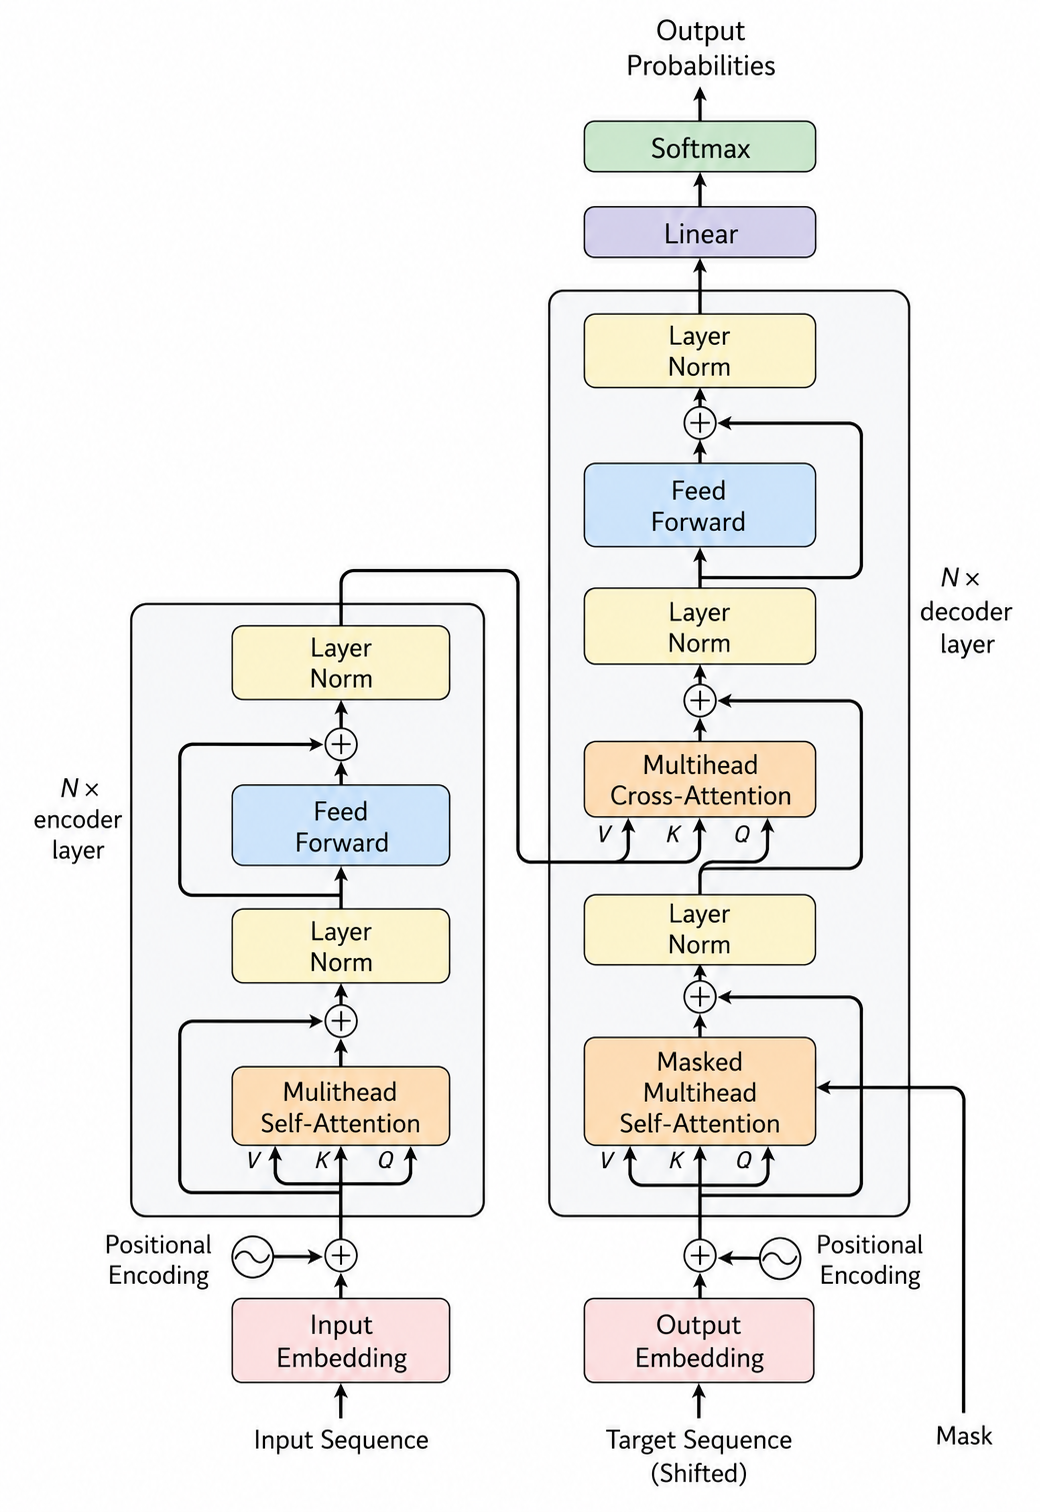
\includegraphics[width=0.6\linewidth]{./chapter2/media/TransformerArchitectur3}
	\caption[Transformer Architecture]{Original Transformer architecture, consisting of an encoder and a decoder part. Image based on:~\cite{Vaswani2017AttentionIA}.}
	\label{fig:TransformerArchitecture}
\end{figure}

While the examples in this section are based on text processing to facilitate understanding of the Transformer architecture, the underlying principles generalize to other modalities, such as images or videos. 



\paragraph{Input Embeddings}
Before a Transformer can process data, the data must be converted into vectors, which is done by the input embedding layer~\cite{Raschka2024BuildLLM}.  Given an input text such as ``Data visualization empowers users to'', the model first tokenizes the text, then maps each token to a vector representation and finally adds positional information~\cite{Raschka2024BuildLLM, TransformerExplainerLLM}. The resulting embedding combines semantic meaning with information about token order. 
\begin{enumerate}
	\item \textbf{Tokenization:} The input text is split into smaller units called tokens. These tokens can be a word, a subword or a single character. For example, the sentence might be tokenized into ["Data", "visualization", "empowers", "users", "to"]. Each token is assigned a unique token ID.
	\item \textbf{Embedding:} Each token is then mapped one-to-one to a high-dimensional vector representation. This embedding captures the semantic meaning of the token. For example, the token "Data" might be represented as a 768-dimensional vector in the embedding space.
	\item \textbf{Positional Encoding:} Since the Transformer does not process tokens sequentially, it needs an explicit way to represent token order. Positional encodings provide this information. Depending on the model, these encodings may be fixed or learned. They are added to the token embeddings so that the model can distinguish between, for example, ``dog bites man'' and ``man bites dog''.
	\item \textbf{Final Embedding:} The final input representation is obtained by combining token embeddings and positional information, typically through element-wise addition. This representation is then passed into the Transformer layers.
\end{enumerate}


\paragraph{Attention Mechanism}
The Attention mechanism is responsible for capturing contextual relationships between tokens by directly computing their relevance to one another. This allows the model to understand long-range dependencies and contextual relationships of the tokens, leading to more coherent and relevant output~\cite{Raschka2024BuildLLM, TransformerExplainerLLM, AttentionTransformersStepbystep}. 
In \autoref{fig:TransformerAttentionWeights} the attention weights of the word ``it'' in the sentence ``The animal didn't cross the street because it was too tired'' are visualized, after the input is processed through the Encoder attention mechanism. The attention weights allows the model to decide which other tokens in the sequence are most relevant. 
% The attention mechanism allows the model to determine that ``it'' refers to ``The animal'' and not to ``the street'' and simultaneously it refers to the context ``too tired'', which is crucial for understanding the meaning of the sentence. 

\begin{figure}
	\centering
	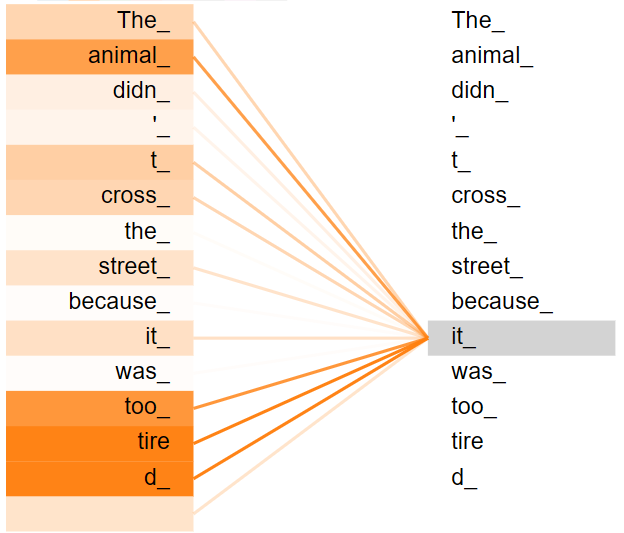
\includegraphics[width=0.4\linewidth]{./chapter2/media/AttentionWords2}
	\caption[Transformer: Attention Weights Example]{Attention Weights of the word ``it'' in a sentence. Image source:~\cite{GoogleColab}}
	% https://colab.research.google.com/github/tensorflow/tensor2tensor/blob/master/tensor2tensor/notebooks/hello_t2t.ipynb#scrollTo=OJKU36QAfqOC.
	\label{fig:TransformerAttentionWeights}
\end{figure}

\textit{Compute Attention Weights.} In the self-attention mechanism, each token embedding vector $\mathbf{x}^{(i)}$ is transformed into three different representations: query $\mathbf{q}^{(i)}$, key $\mathbf{k}^{(i)}$ and value $\mathbf{v}^{(i)}$. These representations are obtained through learnable linear transformations with parameters ($W_q$, $W_k$, $W_v$) that are optimized during training~\cite{Raschka2024BuildLLM, TransformerExplainerLLM, AttentionTransformersStepbystep}.
\begin{itemize}
	\item \textbf{Query $\mathbf{q}^{(i)}=\mathbf{x}^{(i)}\mathbf{W}_q$:} The query vector represents the token for which attention is computed. It is used to determine how much attention this token should pay to other tokens in the sequence.
	\item \textbf{Key $\mathbf{k}^{(i)}=\mathbf{x}^{(i)}\mathbf{W}_k$:} The key vector represents the token against which the query is compared. It is used to compute the relevance score between the query and the token.
	\item \textbf{Value $\mathbf{v}^{(i)}=\mathbf{x}^{(i)}\mathbf{W}_v$:} The value vector contains the actual information of the token. It is weighted by the attention scores to produce the final output of the self-attention mechanism.
\end{itemize}


\textit{Single-Head Self-Attention.}
% \textit{Self-Attention.} 
The query vectors are then compared with the key vectors of all tokens in the sequence using the dot product (scalar product), producing relevance scores that indicate how strongly tokens are related to one another. To stabilize training, these scores are scaled by the square root of the key dimension $d_k$ and normalized using a softmax function, resulting in attention weights. Finally, the attention weights are applied to the corresponding value vectors $\mathbf{v}^{(i)}$ and these weighted values are aggregated to produce the new context vector $\mathbf{z}^{(i)}$ and the output of the self-attention layer~\cite{Raschka2024BuildLLM, TransformerExplainerLLM, AttentionTransformersStepbystep}, see \autoref{fig:TransformerAttentionKeyQueryValueSimply}. 
\begin{equation}
	\mathbf{z}^{(i)} = \text{softmax}\left(\frac{\mathbf{q}^{(i)} \cdot \mathbf{k}^{(i)T}}{\sqrt{d_k}}\right) \cdot \mathbf{v}^{(i)}
\end{equation}
In this way, each token can incorporate information from the most relevant tokens in the sequence, enabling the model to capture contextual dependencies. 
But what does this mean technically? The value vector $\mathbf{v}^{(i)}$ represents the token's information in a semantically learned high-dimensional embedding space. Through the attention mechanism, the vector's direction and magnitude in this embedding space are adjusted, resulting in a different semantic meaning.
In \autoref{fig:TransformerEmbeddingSpace_BlueFluffyCreature4}, it is shown how the vector of the word ``creature'' is shifted in the embedding space based on the context ``a fluffy blue creature''. This illustrates how the attention mechanism allows the model to dynamically adjust the meaning of tokens based on their relationships with other tokens in the sequence~\cite{AttentionTransformersStepbystep}.
% In one context, it may point to a specific type of creature, while in another context, it may point to a different type of creature.
% According to the relevant semantic meaning, the word “creature” is affected within the vectorial embedding space by the words (embeddings) “fluffy” and “blue”
\begin{figure}[!h]
	\centering
	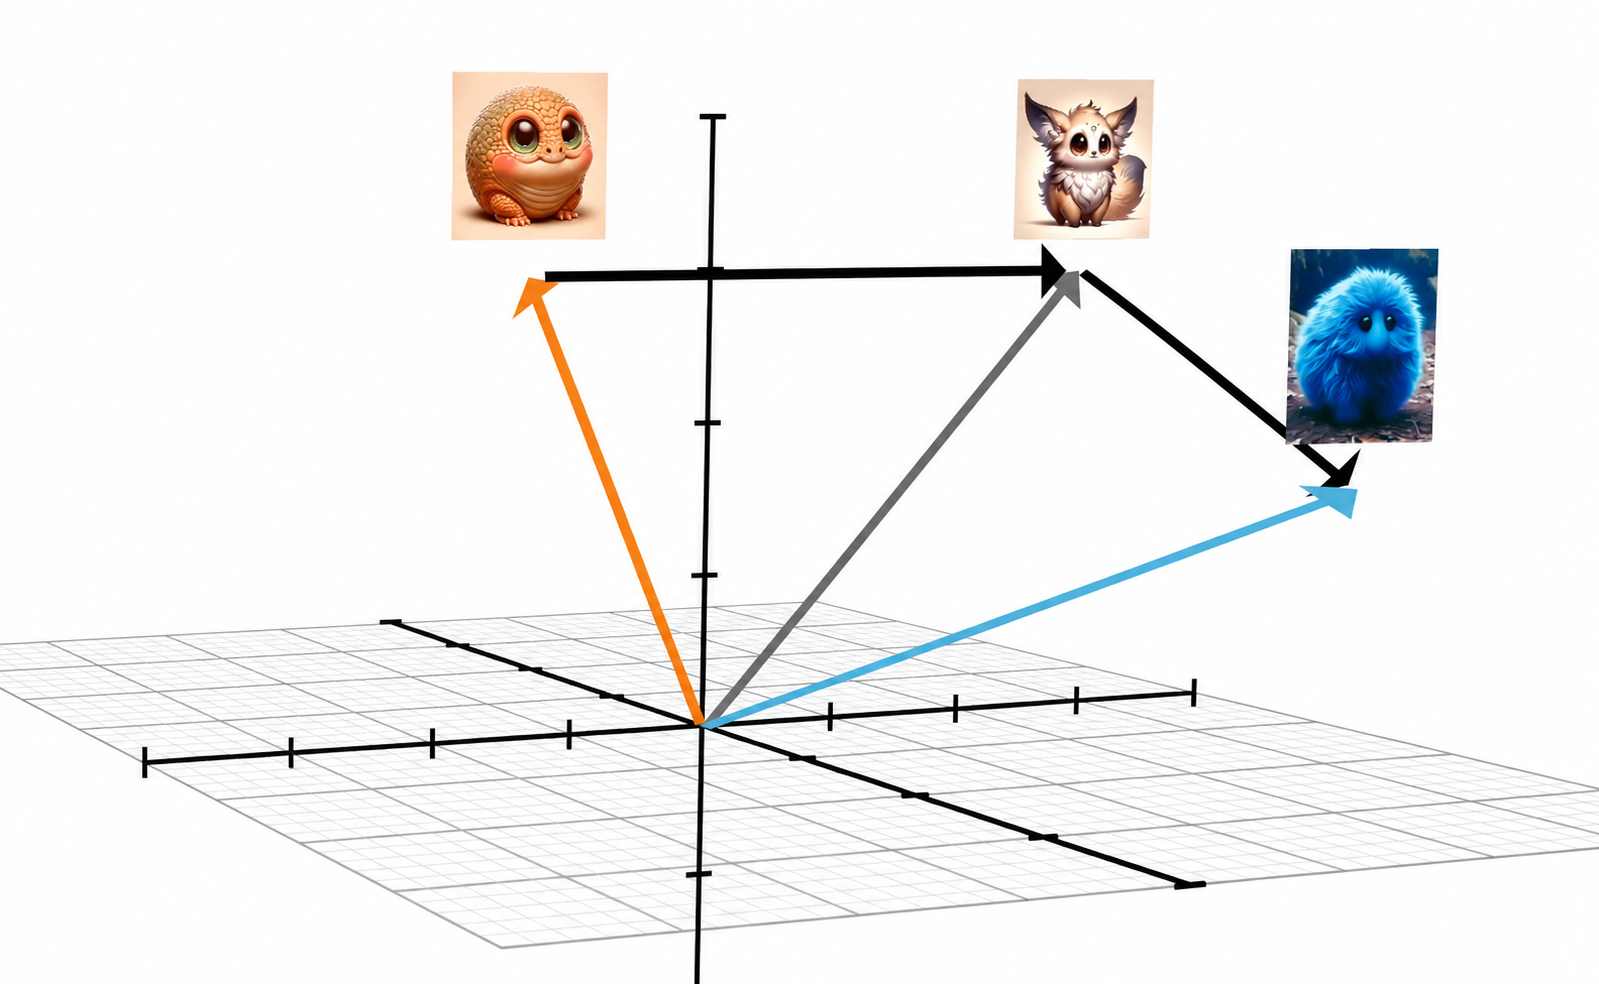
\includegraphics[width=0.6\linewidth]{./chapter2/media/TransformerEmbeddingSpace_BlueFluffyCreature4}
	\caption[Transformer: Embedding Space]{Illustration of the value embedding space $V$: The vector of ``creature'' is shifted in the embedding space based on the context ``a fluffy blue creature''. Image source:~\cite{AttentionTransformersStepbystep}.}
	\label{fig:TransformerEmbeddingSpace_BlueFluffyCreature4}
\end{figure}
% are weighted by the attention scores, allowing each token to aggregate information from other tokens based on their relevance.

\begin{figure}
	\centering
	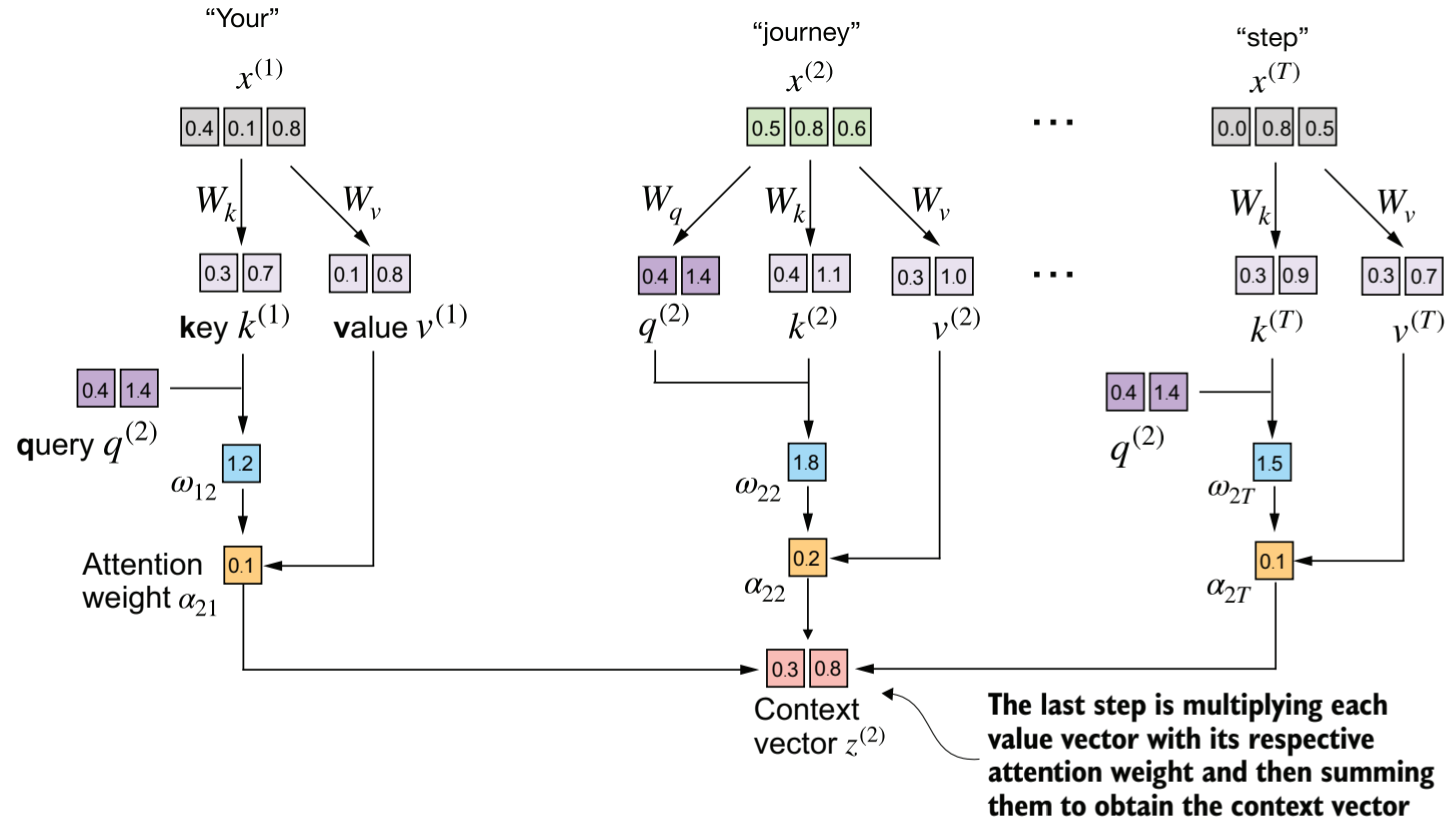
\includegraphics[width=1.0\linewidth]{./chapter2/media/TransformerAttentionKeyQueryValueSimply}
	\caption[Transformer: Self-attention computation]{Self-attention: Compute the new context vector of each input embedding vector by combining the (attention)-weighted value vectors. Image source:~\cite{Raschka2024BuildLLM}.}
	\label{fig:TransformerAttentionKeyQueryValueSimply}
\end{figure}

Instead of computing attention separately for each token, the Transformer performs the computation for the entire sequence using matrix operations~\cite{Raschka2024BuildLLM}, see \autoref{fig:TransformerSingleHeadAttention}. The matrix product $\mathbf{QK}^T$ computes the pairwise similarity scores between all tokens in the sequence in parallel, resulting in the attention score matrix.
\begin{equation}
	\mathbf{Z} = {Attention}(\mathbf{Q},\mathbf{K},\mathbf{V})=\text{softmax}\left( \frac{\mathbf{QK}^T}{\sqrt{d_k}} \right)\mathbf{V}
\end{equation}

\begin{figure}
	\centering
	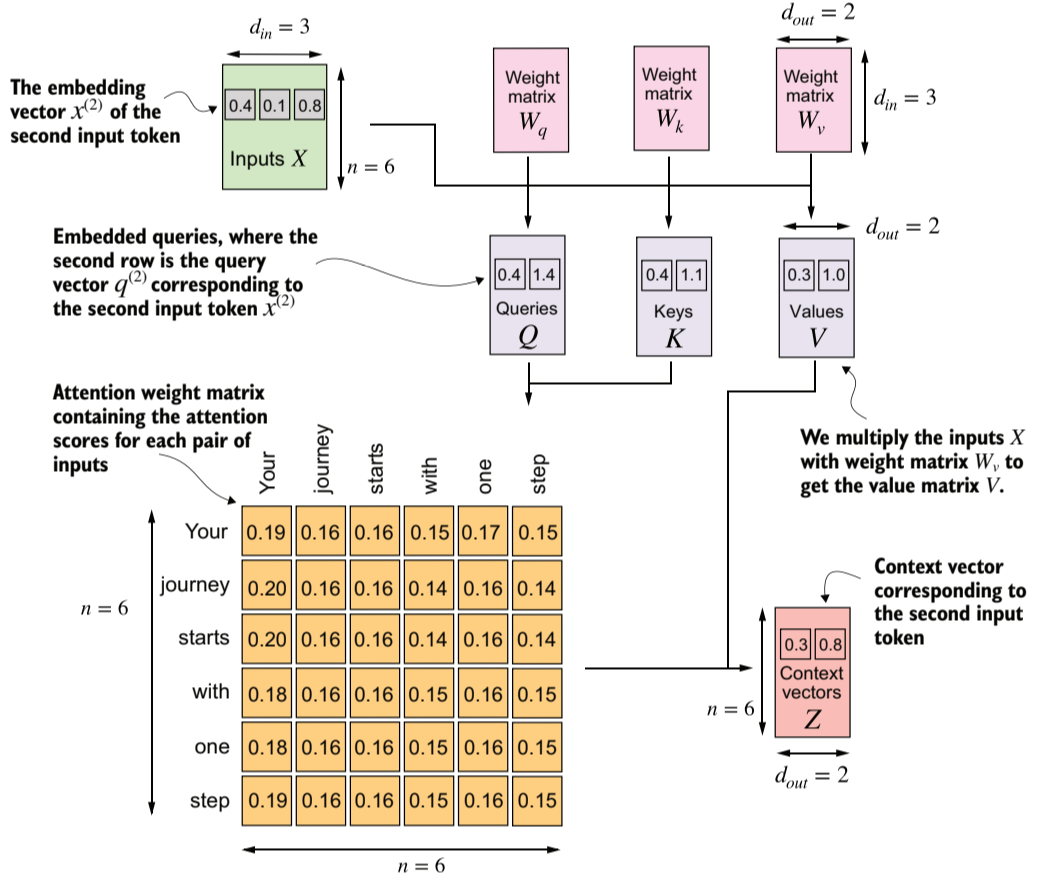
\includegraphics[width=0.8\linewidth]{./chapter2/media/TransformerSingleHeadAttention}
	\caption[Transformer: Self-attention computation]{Overview of a single self-attention block. Image source:~\cite{Raschka2024BuildLLM}.}
	\label{fig:TransformerSingleHeadAttention}
\end{figure}

% \paragraph{Multi-Head Self-Attention}
\textit{Multi-Head Self-Attention.} 
While a single attention mechanism can capture relationships between tokens, different types of dependencies may exist simultaneously within a sequence. To address this, the Transformer employs multi-head attention, which consists of several attention heads operating in parallel~\cite{Raschka2024BuildLLM, Vaswani2017AttentionIA}. Each head learns its own query, key and value projections and therefore focuses on different aspects of the input data. For example, one head may capture syntactic relationships, while another focuses on semantic dependencies. The outputs of all heads are concatenated and projected through a linear layer to form the final representation, see \autoref{fig:TransformerMultiHeadAttention}. This increases the model's ability to learn diverse linguistic patterns and contextual relationships.

\begin{figure}
	\centering
	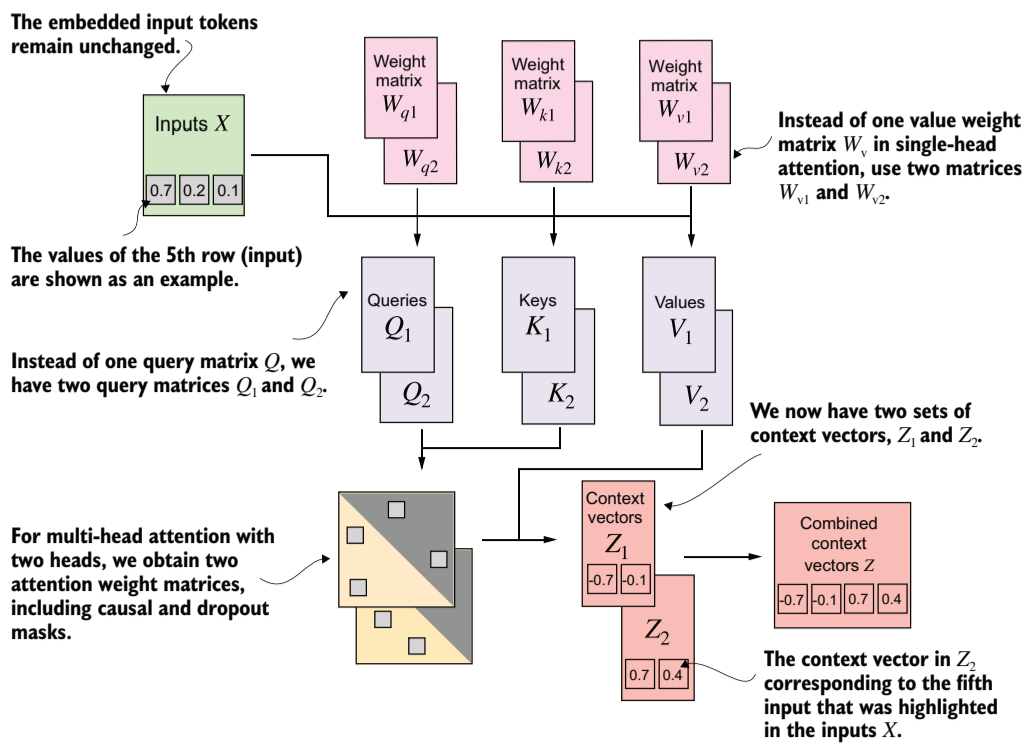
\includegraphics[width=0.8\linewidth]{./chapter2/media/TransformerMultiHeadAttention}
	\caption[Transformer: Multi-Head Attention Block]{Overview of a multi-head attention block. Image source:~\cite{Raschka2024BuildLLM}.}
	\label{fig:TransformerMultiHeadAttention}
\end{figure}


\paragraph{Encoder Block}
After the self-attention computation, the resulting representations are passed through a layer normalization step, followed by a \ac{MLP} Network. A second layer normalization is applied after this transformation. This sequence of operations forms a single Transformer block, which can be stacked multiple times to increase model capacity~\cite{Vaswani2017AttentionIA}.
The \ac{MLP} operates independently on each token representation. 
% In contrast to the attention mechanism, which is responsible for exchanging information between tokens, the \ac{MLP} refines and transforms each token embedding individually. 
It typically consists of two linear transformations with a non-linear activation function in between, allowing the model to learn more complex feature transformations.
A key component of the Transformer architecture is the use of residual connections, which are applied around both the attention block and the feed forward network and add the input of a sub-layer directly to its output~\cite{Vaswani2017AttentionIA}. This improves gradient flow during backpropagation and mitigates the vanishing gradient problem, which is especially important in deep networks composed of many stacked Transformer blocks. 

The output of the final encoder layer is a sequence of contextualized vectors, where each vector corresponds to one input token enriched with information from the entire sequence. This representation can then be used for downstream tasks such as classification, regression, or sequence generation.


\paragraph{Decoder Block}
The decoder receives an input sequence that is first transformed using the same embedding procedure as the encoder (token embeddings + positional information)~\cite{Vaswani2017AttentionIA}. During generation, this input typically consists of previously generated output tokens. The embedded sequence is then processed through two distinct attention mechanisms: masked multi-head self-attention and cross-attention.
% \paragraph{Masked Multi-Head Attention}
% \textit{Masked Multi-Head Attention.} 
Masked multi-head self-attention operates on the decoder's own input sequence, but with a causal mask that prevents each position from attending to any future positions~\cite{Raschka2024BuildLLM}. This ensures that every generated token depends only on its previous tokens.

In cross-attention, the decoder's hidden states from the masked attention layer serve as queries $Q$, while the encoder's output serve as keys $K$ and values $V$, allowing the decoder to condition its predictions on the encoded source sequence~\cite{Vaswani2017AttentionIA}.

After these attention layers, the resulting representations are passed through a linear projection head followed by a softmax function, producing a probability distribution over the set of possible output elements~\cite{Vaswani2017AttentionIA, Raschka2024BuildLLM, TransformerExplainerLLM}. The element with the highest probability (in our case the vocabulary token) is selected and appended to the generated sequence. This process repeats autoregressively until a special end-of-sequence symbol is produced. 
% In our text example, the vocabulary token with the highest probability is selected and appended to the generated sequence.







\section{Vision Transformer}
The Vision Transformer (ViT)~\cite{Dosovitskiy2020AnII} extends the Transformer architecture, originally developed for natural language processing, to computer vision tasks by applying the self-attention mechanism to image patches instead of words. In computer vision, attention enables a model to focus on relevant regions of an image and to capture and understanding relationships between different areas of an image. This allows the model to identify important objects and effectively model spatial dependencies across the entire image.

\begin{figure}[!h]
	\centering
	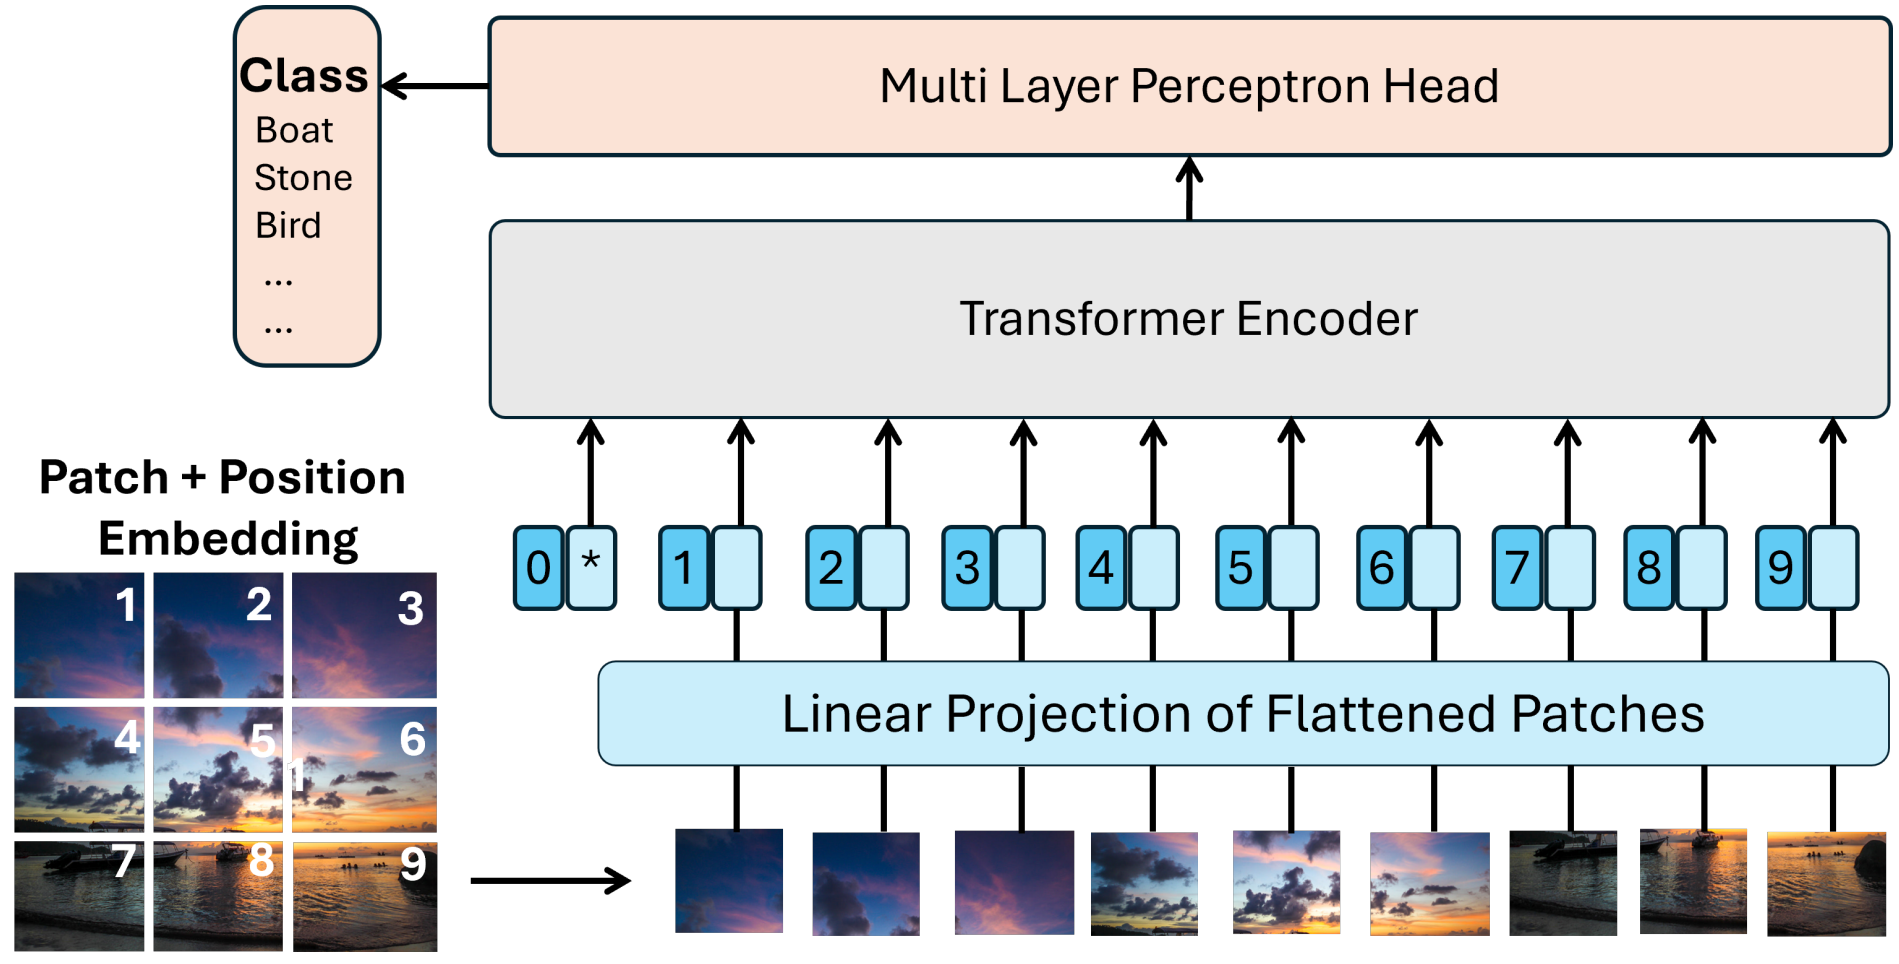
\includegraphics[width=0.6\linewidth]{./chapter2/media/VisionTransformerOverview}
	\caption[Vision Transformer Overview]{Vision Transformer: Overview of the architecture. Image source~\cite{Din2025VisionLA}.}
	\label{fig:VisionTransformerOverview}
\end{figure}

To process an image, ViT first divides the input image into a sequence of fixed-size, non-overlapping patches, see \autoref{fig:VisionTransformerOverview}. Each patch is flattened and linearly projected into a fixed-dimensional embedding vector, analogous to token embeddings in natural language processing.
Since the Transformer architecture does not inherently encode spatial information between the image patches, learnable positional embeddings are added to these patch embeddings. In addition, a learnable classification token (CLS token), denoted by an asterisk (*) in \autoref{fig:VisionTransformerOverview}, is prepended to the sequence and serves as a global representation of the whole image. During the attention computation, the CLS token interacts with all patch embeddings and gradually aggregates information from the entire image.
The resulting sequence is processed by a standard Transformer encoder consisting of multi-head self-attention and feed-forward layers. 
% Through self-attention, the model learns global relationships between image patches and can capture long-range spatial dependencies that are difficult to model with traditional CNN approaches. 
After the final encoder layer, the output representation of the CLS token serves as a global representation of the image and is passed through a multi-layer perceptron (MLP) head to generate the final prediction, such as class probabilities for image classification tasks.
% After the final encoder layer, the output representation of the CLS token contains information aggregated from all image patches and is passed to a multi-layer perceptron (MLP) head to produce the final prediction

Vision Transformers have demonstrated competitive performance on large-scale image classification benchmarks such as ImageNet~\cite{Deng2009ImageNetAL}, highlighting the effectiveness of attention-based architectures for visual representation learning~\cite{Dosovitskiy2020AnII}.
In imitation learning, Vision Transformers can be used as visual encoders that extract global scene representations from camera observations, which are subsequently used by the policy network to predict actions.







\section{Foundation Model}


% Recent advances in artificial intelligence have been largely driven by the development of foundation models. 
A foundation model is a large-scale model that is pre-trained on vast amounts of data and can subsequently be adapted to a wide range of downstream tasks~\cite{Bommasani2021OnTO}. Instead of being designed for a single application, foundation models learn general patterns, concepts and representations that can be reused across different domains and tasks.
A key characteristic of foundation models is their ability to generalize to problems that were not explicitly specified during training. This broad knowledge enables them to serve as a common basis for many specialized applications. 
Unimodal foundation models (e.g. GPT-3 for text~\cite{Brown2020LanguageMA}, Stable Diffusion for images~\cite{Rombach2021HighResolutionIS}) learn patterns within a single data type, whereas Multi-modal foundation models (e.g. CLIP~\cite{Radford2021LearningTV}, GPT-4V~\cite{Achiam2023GPT4TR}, Gemini~\cite{Reid2024Gemini1U, team2023gemini}) learn joint representations across modalities such as text, images and audio.
Due to their versatility and strong generalization capabilities, foundation models have become the foundation of many modern \ac{AI} systems.


% \begin{figure}[!ht]
% 	\centering
% 	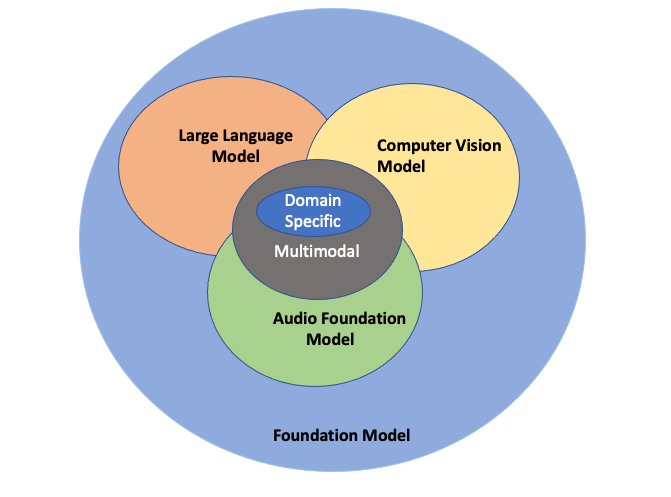
\includegraphics[width=0.55\linewidth]{./chapter2/media/FoundationModel_vs_MultiModalModel.png}
% 	\caption[Foundation Model vs. Multi-Model Model]{Foundation Model vs. Multi-Model Model. Image source:~\cite{FoundationModelsFoundation}}
% 	\label{fig:foundationmodel_vs_multimodel}
% \end{figure}

\section{Multi-Modal Model}
A multimodal model is capable of processing and relating information from two or more data modalities, such as text, images, audio, or sensor measurements~\cite{Baltruaitis2017MultimodalML}. Unlike unimodal models, which operate on only a single type of data, multimodal models learn a shared representation that enables information from different modalities to be interpreted jointly.
The integration of multiple modalities allows a model to leverage complementary information, handle missing data from one source by relying on another, provide more comprehensive insights and improves model generalization~\cite{Liang2022FoundationsT}.
For example, a multimodal model can analyze an image together with a textual instruction and use information from both inputs to answer a question or perform a task. 
Multimodal Learning is a own learning paradigm and refers to the use of various data modalities within a single learning concept~\cite{Ngiam2011MultimodalDL, Baltruaitis2017MultimodalML}.







\section{Reinforcement Learning} \label{sec:ReinforcementLearning}
\ac{RL} is both a fundamental discipline of \ac{ML} and a distinct approach within Robot Learning.
The robot learns a policy through trial and error using rewards provided from the given task and the environment. The actions performed by the agent are evaluated with a reward score and this score is then used to gradually optimize the policy. See also figure \ref{fig:RLConzept} for a general graphical overview. Below are the key terms in \ac{RL} explained in relation to robotics: 
\begin{itemize}
	\item \textbf{Agent:} The agent is the entity that learns to perform a specific behavior through interaction with its environment. In the context of this work, the agent corresponds to the robot, which has to execute a given action or task. 
	\item \textbf{Environment:} The environment is the setting in which the agent operates and is the workplace of the robot. In addition to the robot itself, it includes all relevant objects with which the robot interacts. The environment can be a simulated environment too.
	\item \textbf{Robot Actions $a$:} The Robot actions are simply the control commands the robot sends to its actuators, e.g. open or close the gripper, move to position $X,Y,Z$, joint angles, etc.
	\item \textbf{Reward $r$:} The reward is a numerical value that indicates how well the robot is performing in relation to the task objective. If the robot successfully picks up an object, it might receive a positive reward, while if it fails or drops the object, it might receive a negative reward. The goal of Reinforcement Learning is to learn a policy that maximizes the cumulative reward over time.
	\item \textbf{Robot State $s$:} The State is a complete description of the situation in the environment at a particular point in time. 
	% The robot state represents the current situation of the robot and its environment. 
	It can include various types of information, such as the robot's position, orientation, joint angles, sensor readings and even visual input from cameras~\cite{walkerastroActionSpaceState2024}. The state is crucial for the robot to make informed decisions about which actions to take.
	\item \textbf{Observation $o$:} An observation is the information that the robot receives from its sensors at a given time step. It may not provide a complete picture of the environment and thus may not fully represent the true robot state. In our case, the observation is mostly equivalent to the state~\cite{walkerastroActionSpaceState2024}. The observation can for example include the last camera frames as well as additional sensor inputs such as proprioceptive signals from the robot.
	\item \textbf{Policy $\pi$:}
	The policy can be interpreted as the brain of the agent and controls the robot's motion. The policy determines which action should be taken next when the agent is in a particular state in order to achieve the task objective. 
	% The Policy controls the robot's motion and actions. 
	Formally, a policy can be represented as  
	\begin{align}
		\pi_\theta(a \mid s)  
	\end{align}
	which defines a probability distribution over actions $a$, conditioned on the current state $s$. In other words, the policy specifies how likely the agent is to select a particular action given its current observation of the environment. 

\end{itemize}





\paragraph{Markov Decision Process}

\ac{RL} is based on the \ac{MDP}. A \ac{MDP} is a stochastic decision-making process that formally models the transition probabilities from a state $s$ to a subsequent state $s'$ provided that action $a$ is performed, expressed mathematically as $P(s'|s,a)$~\cite{sutton2018reinforcement, millerMarkovDecisionProcesses}. 
The objective is to learn a policy $\pi(a|s)$ that maximizes the expected long-term cumulative reward, defined as $\mathbb{E}\left[\sum_{t=0}^{\infty} \gamma^t r_t\right]$. The discount factor $\gamma \in [0,1]$ determines the importance of future rewards compared to immediate rewards. A value of $\gamma$ close to 0 makes the agent focus more on immediate rewards, while a value close to 1 encourages the agent to consider long-term rewards more heavily~\cite{sutton2018reinforcement, jagtapUnderstandingMarkovDecision}.
A \ac{MDP} also defines the reward function $R_a(s,s')$ that specifies the reward $r$ an agent receives when taking action $a$ in state $s$ and transitioning to a subsequent state $s'$~\cite{sutton2018reinforcement, millerMarkovDecisionProcesses}.
%  This is commonly expressed as $R_a(s,s')$~\cite{sutton2018reinforcement, millerMarkovDecisionProcesses}.

The \textbf{Markov property} says that all information from the past is contained in the current state, mathematically expressed as $P(s_{t+1}|s_{t}) = P(s_{t+1}|s_{1},s_{2}, ... s_{t})$. In other words, the transition probabilities depend only on the current state and not on the history of previous states~\cite{jagtapUnderstandingMarkovDecision}.
In practice, the Markov property is often not strictly satisfied. For example, a single image captured by a camera does not provide sufficient information to infer the dynamics of the environment. From one image alone, it is not possible to determine whether a car is moving forward at 100 km/h or 10 km/h, reversing, or remaining stationary. However, such information is crucial for making correct decisions in applications like autonomous driving~\cite{staffWhatMarkovDecision2025}.
Therefore, in practice, only sufficiently informative state representations are often used because the ideal Markov property is not strictly fulfilled. In the example above, the sequence of the last camera frames can be used.
%  to better capture the underlying dynamics of the environment~\cite{millerMarkovDecisionProcesses}.



\paragraph{Training Process}
At the beginning of the training process, a randomly initialized policy leads the robot to perform random movements. Through this interaction with the environment, the agent explores different actions and attempts to identify those that yield high rewards. Actions associated with higher rewards are subsequently assigned a higher probability by the policy, making the robot more likely to select them in similar situations in the future.

A successful learning process requires a suitable balance between exploration and exploitation. 
Exploration involves trying new or infrequently selected actions to gather information about the environment, while exploitation focuses on selecting actions that have previously yielded high rewards. Early in training, exploration is emphasized to discover effective behaviors, whereas later stages increasingly rely on exploitation to maximize task performance.

Numerous methods and algorithms have been proposed to effectively balance exploration and exploitation, $\epsilon$-greedy strategy, Upper Confidence Bound (UCB) and Thompson Sampling. 
% However, a detailed discussion of these methods is beyond the scope of this thesis.
Due to the exploration phase, the success of the chosen \ac{RL} approach only becomes visible at a late stage, unlike in classical deep learning, see Figure \ref{fig:trainingprogressdlandrl}. 


\begin{figure}[!ht]
	\centering
	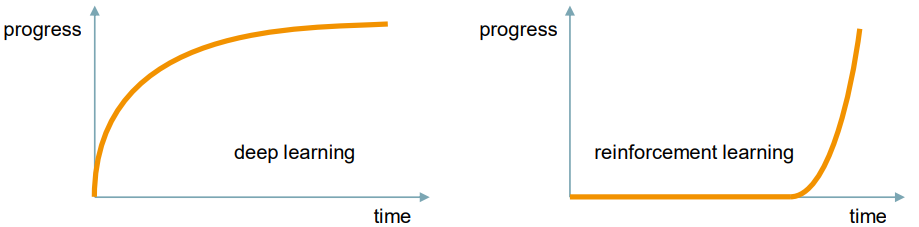
\includegraphics[width=0.7\linewidth]{./chapter3/media/TrainingProgressDLandRL.png}
	\caption[Training Progress in Deep Learning and Reinforcement Learning]{The task success in \ac{RL} becomes visible at a later stage compared to deep learning due to the exploration phase. Image source:~\cite{KontaktNierhoff}}
	\label{fig:trainingprogressdlandrl}
\end{figure}











% \subsection{Knowledge Modalities from Video}
\paragraph{Knowledge Modalities from Video}
An \ac{RL} \ac{KM} is some function learned from data that represents specific types of \ac{RL}-related knowledge.
\ac{KM}s can be learned through trial-and-error principles or from video datasets~\cite{Wulfmeier2023FoundationsFT}:
%  can capture different aspects of the \ac{RL} problem~\cite{Wulfmeier2023FoundationsFT}. 

\begin{itemize}
	\item \textbf{Policy:} The policy specifies how likely the agent is to select a particular action given its current observation of the environment.
	It can be learned from video data by observing the actions taken in different states and learning to predict those actions based on the visual input~\cite{Wulfmeier2023FoundationsFT}. 
	
	\item \textbf{Value functions:} Value functions estimate the expected future return (cumulative reward) for a given state~\cite{sutton2018reinforcement}, see Figure \ref{fig:VFunctionVsQFunction}. They can be learned from video data by observing the outcomes of actions and learning to predict the expected future rewards based on the visual input~\cite{Wulfmeier2023FoundationsFT}.

	\begin{itemize}
		% V-Function
		\item \textit{State-value function (V-function):} 
		A V-function $V_\pi(s_t)$ is a mapping from states to the expected future return when acting under a particular policy $\pi$~\cite{sutton2018reinforcement}. $V_\pi(s)$ does not provide information about the quality of individual actions available in that state $s$. 
		Intuition: ''How good is it to be a certain state, if I follow my policy $\pi$?''

		% \begin{figure}[!ht]
		% 	\centering
		% 	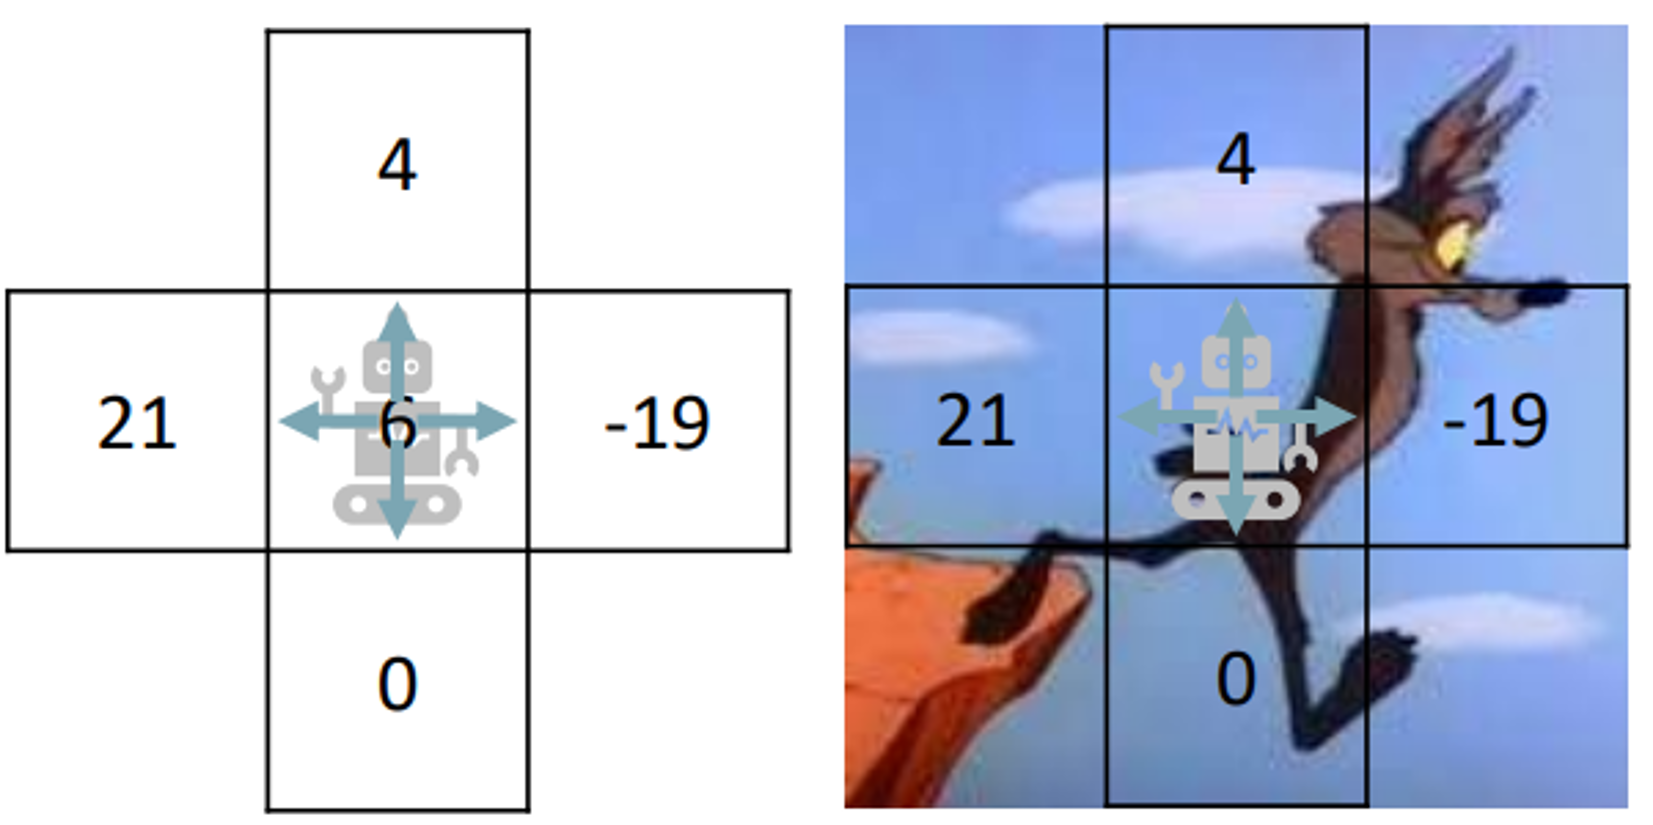
\includegraphics[width=0.55\linewidth]{./chapter3/media/V_Function.png}
		% 	\caption[State-Value Function]{State-Value Function}
		% 	\label{fig:statevaluefunction}
		% \end{figure}

		% Q-Function
		\item \textit{State-action value function (Q-function):} 		
		A Q-function $Q_\pi(s_t,a_t)$ is a mapping from state-action pairs to the expected future return when acting under a particular policy $\pi$~\cite{sutton2018reinforcement}. $Q_\pi(s,a)$ evaluates the expected return of taking a specific action $a$ in state $s$ and subsequently following the policy $\pi$. It provides information about the quality of individual actions available in that state $s$.
		Intuition: ''How good is this specific action in a certain state, if I continue behaving like my policy $\pi$?''

		% \begin{figure}[!ht]
		% 	\centering
		% 	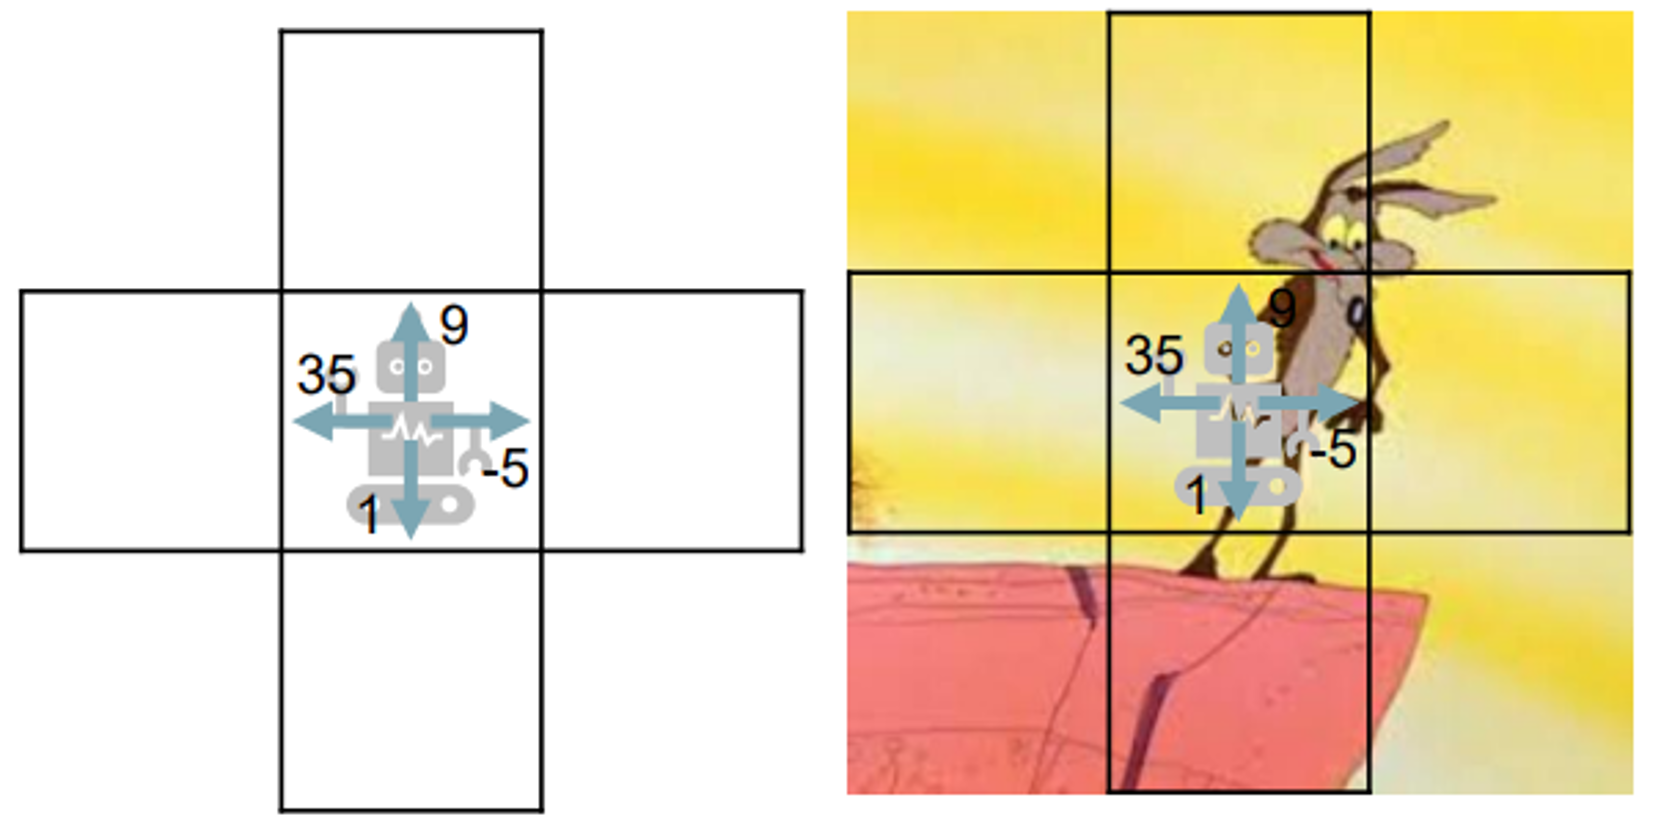
\includegraphics[width=0.55\linewidth]{./chapter3/media/Q_Function.png}
		% 	\caption[State-Action Value Function]{State-Action Value Function}
		% 	\label{fig:stateactionvaluefunction}
		% \end{figure}

		

	\end{itemize}
	
	\begin{figure}[h]
		\centering
		\subfigure[V-Function: Returns the expected future return for a given state.]{
				\begin{minipage}{6.3cm} % subfigure box width
				\centering
				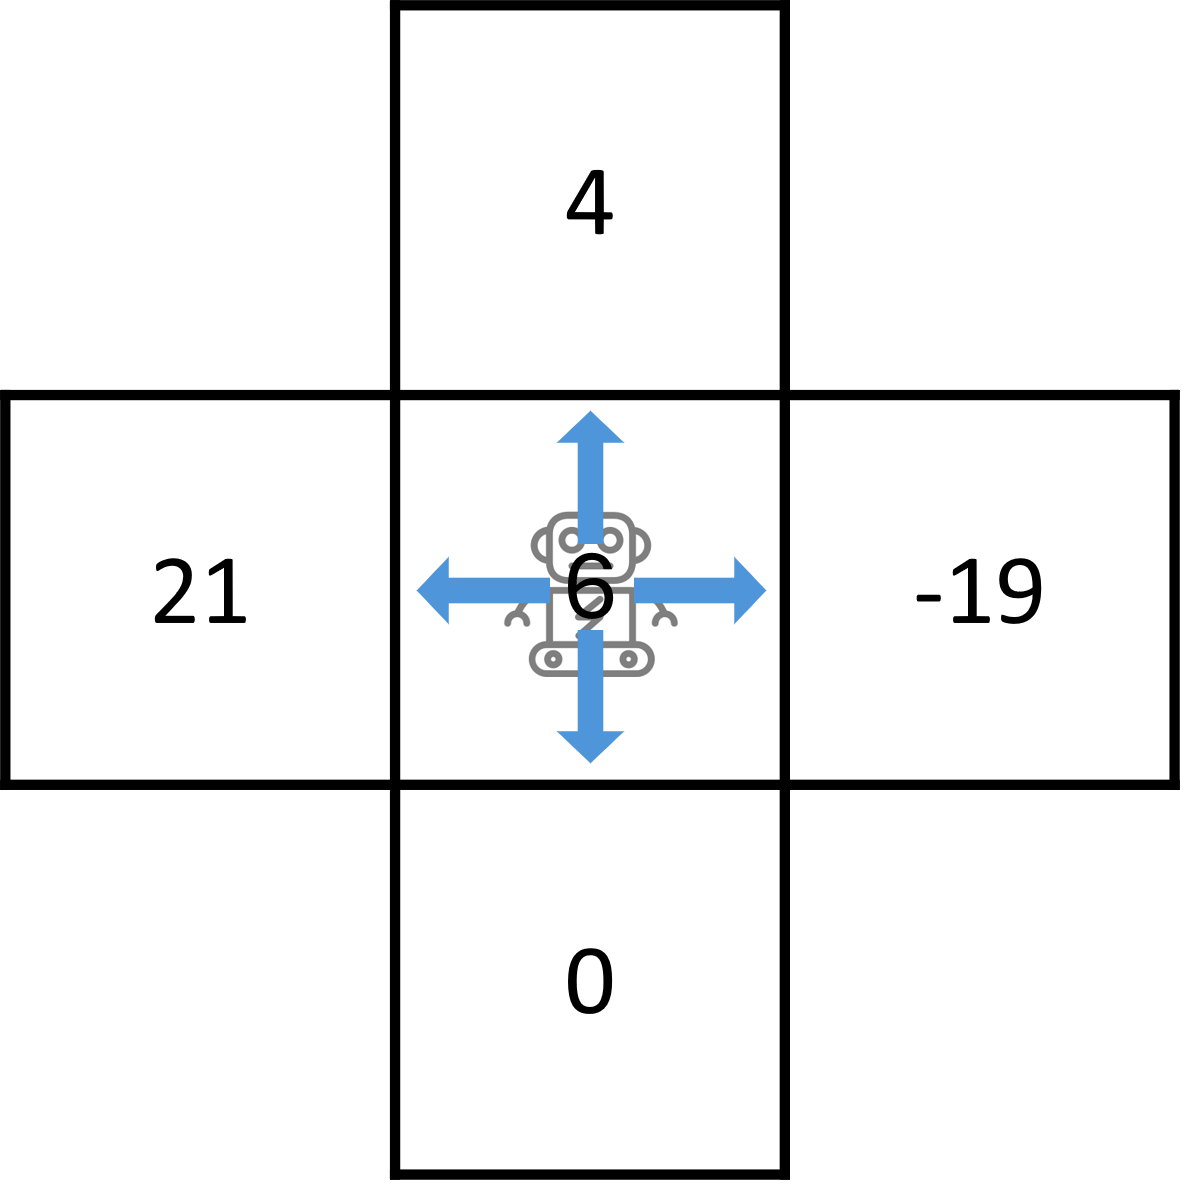
\includegraphics[width=4.6cm]{./chapter2/media/RL_VFunction.png}
				\label{fig:RL_VFunction}
			\end{minipage}%
		}
		\hspace{0.8cm}
		\subfigure[Q-Function: Returns the expected future return for a given state-action pair.]{
			\begin{minipage}{6.3cm} % subfigure box width
				\centering
				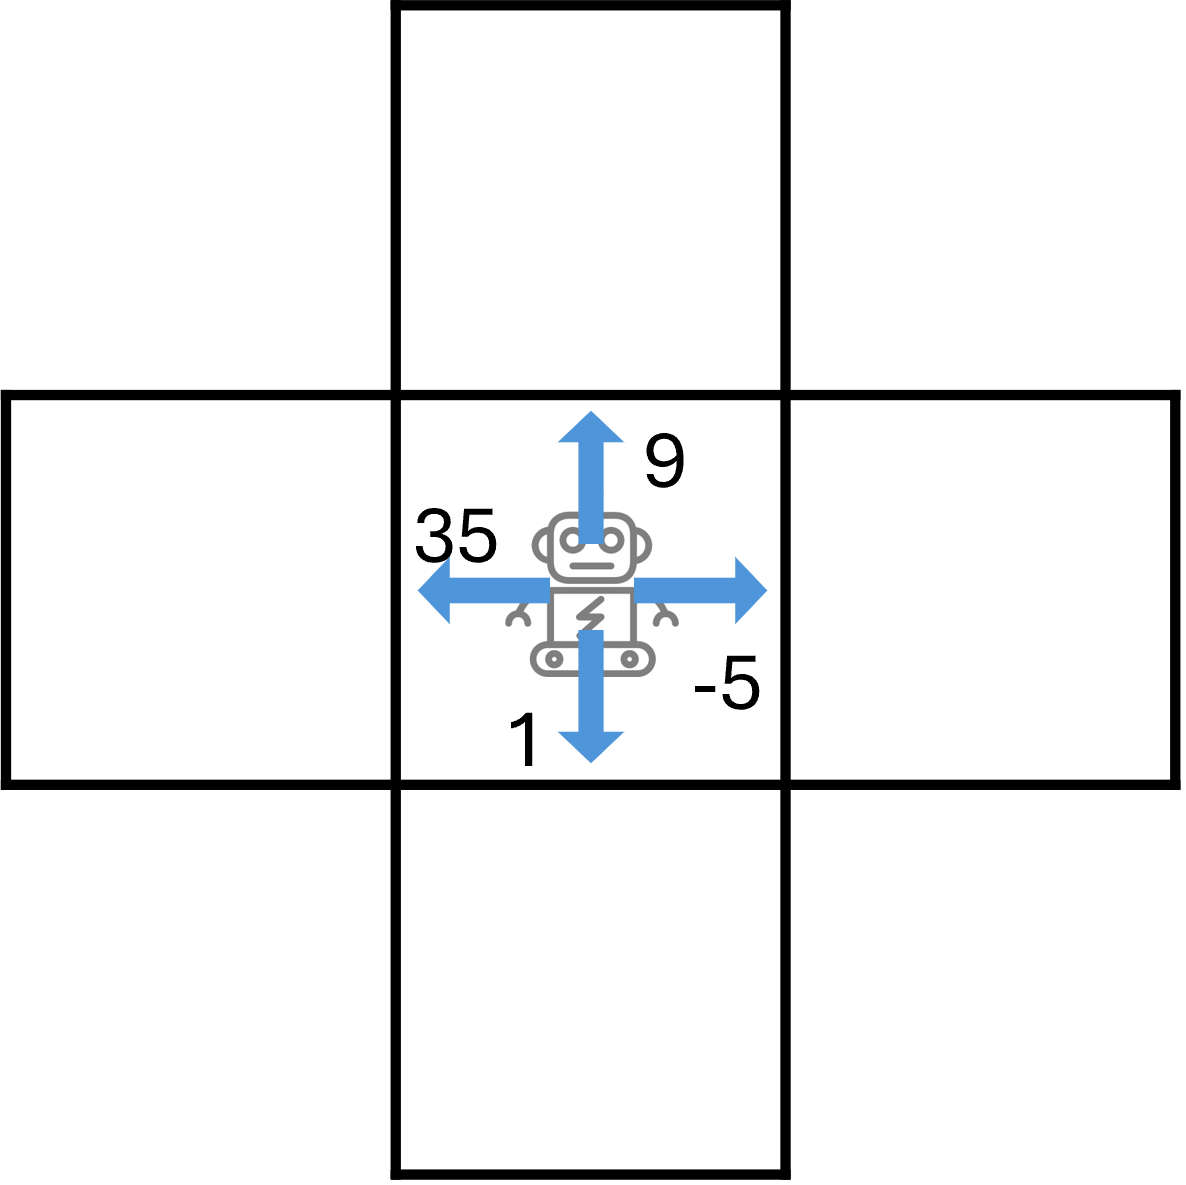
\includegraphics[width=4.6cm]{./chapter2/media/RL_QFunction.png}
				\label{fig:RL_QFunction}
			\end{minipage}%
		}
		\caption[Comparison of V-Function and Q-Function.]{Comparison of V-Function and Q-Function. The V-Function estimates the expected return for a given state, while the Q-Function estimates the expected return for a given state-action pair. Image based on~\cite{KontaktNierhoff}}
		\label{fig:VFunctionVsQFunction}
	\end{figure}


	% Dynamics model:
	\item \textbf{Dynamics model:} A Dynamics model $p(s_{t+1}|s_t,a_t)$ predicts the next state $s_{t+1}$ given the current state $s_t$ and action $a_t$~\cite{sutton2018reinforcement}. 
	% Video prediction models can be used as robot dynamics models~\cite{Eze2024LearningBW}. 
	By learning to predict future video frames based on current observations and actions, the model can capture the underlying dynamics of the environment and allows the robot to anticipate the consequences of its actions and make informed decisions based on predicted future states~\cite{Eze2024LearningBW}.
	% Reward model:
	\item \textbf{Reward model:} A reward function $r(s_t,a_t)$ defines the reward received by the agent for taking action $a_t$ in state $s_t$~\cite{sutton2018reinforcement}. It can be learned from video data by observing the outcomes of actions and inferring the underlying reward structure that motivates those actions. For example, if a video shows a robot successfully picking up an object, the reward function can learn to assign a positive reward to that action in similar states.
\end{itemize}





\section{Imitation Learning} \label{sec:ImitationLearning}
\ac{IL} or Learning from Demonstration is a general term for methods in which the agent derives or learns its behavior from expert demonstrations or ``in the wild'' videos~\cite{Chrysomallis2025ImitationLI}. ``In the wild'' videos refer to videos that are not specifically recorded for training purposes, but are instead sourced from real-world settings, such as those found in great variety on the internet, for example on platforms like YouTube.
% \ac{IL} makes it possible to use "in the wild" videos—such as those found in great variety on the internet, for example on platforms like YouTube — to train \ac{AI} models~\cite{McCarthy_2025}.
The demonstration videos can show a robot, a human, or even a loose sequence of actions, both in the real world or in a simulation environment, performing a specific task. However, videos without a clearly defined objective or with unknown activity can also be used~\cite{McCarthy_2025}.
Models can through \ac{IL} be trained to capture the visual and semantic relationships, as well as the physical dynamics of the real world. This in turn is a key prerequisite for the development of a generalist policy. 
\ac{IL} can be divided into Behavior Cloning (\autoref{sec:BehaviorCloning}) and Learning from Videos (\autoref{sec:LearningfromVideos}).


\paragraph{Idea Behind Imitation Learning} 
When people want to learn a new skill, they often turn to how-to videos. They learn the new skill through speech instructions and visual observations in the video~\cite{Jain2024Vid2RobotEV}. The same principle is now to be applied to robots through \ac{IL}.
Visual Imitation Learning is particularly well suited for teaching tasks that are difficult or impossible to specify through language alone.
It allows robots to infer task-relevant actions from demonstrations performed in different environments and can be more data-efficient than \ac{RL}, especially in high-dimensional state spaces and complex environments. Furthermore it benefits from large-scale human demonstration datasets, which are often easier to collect than robot-specific expert demonstrations in the specific domain\cite{Jain2024Vid2RobotEV}.
% Visual Imitation Learning ...
% \begin{itemize}
%     \item is ideal for teaching tasks that are difficult or impossible to describe in words.
%     \item allows robots to infer tasks from expert demonstrations in different environments than the robot.
%     \item can be more data efficient than \ac{RL}, especially in high-dimensional state spaces, like a complex robot environment. 
%     \item can leverage large datasets of human demonstrations, which are often easier to collect than expert demonstrations in the specific domain~\cite{Jain2024Vid2RobotEV}.
% \end{itemize}

% \texttt{Problems in RL:}
In \ac{RL} a task is commonly defined through a reward function, which assigns a high reward to desirable behavior and a low reward to undesirable behavior~\cite{sutton2018reinforcement}. However, designing good reward functions is challenging for every task and many methods based on computer vision rely on annotated demonstrations in every new environment~\cite{McCarthy_2025}. \ac{IL} allows us to learn complex behaviors that are difficult to specify through a reward function, or it can help us to define a good adaptive reward function for \ac{RL}.


\subsection{Behavior Cloning}
\label{sec:BehaviorCloning}
\ac{BC} is a fundamental approach within \ac{IL}, where a policy is learned directly from annotated expert demonstrations~\cite{Eze2024LearningBW}. The training data consists of state-action pairs $(s_t, a_t)$ and the problem is formulated as a standard supervised learning task.  
Conceptually, \ac{BC} can be understood as a form of direct imitation or copying of expert behavior, without explicitly modeling the underlying system dynamics or task objectives. 
% Due to its simplicity and scalability, BC is one of the most widely used methods in robot learning from datasets.  
% BC is used to train Vision Language Action models and for pre-training models used in \ac{RL}, see Section \textbf{XXX}

% \paragraph{Purpose: Policy Learning} 
Formally, \ac{BC} learns a policy $\pi_\theta(a_t \mid s_t)$ by supervised learning on expert demonstrations.
% :
% \begin{align}
% 	\pi_\theta(a_t \mid s_t)
% \end{align}
% where:
% \begin{itemize}
% 	\item $s_t$: State / Observation (images, proprioception, etc.) at time $t$
% 	\item $a_t$: Expert action at time $t$
% \end{itemize}
The Policy is optimized by minimizing the prediction error between the actions generated by the model and the corresponding expert actions;
\begin{equation}
	\min_{\theta} \mathbb{E}_{(s_t,a_t) \sim \mathcal{D}} \left[ \mathcal{L}(\pi_{\theta}(s_t), a_t) \right]
\end{equation}
where $\mathbb{E}_{(s,a) \sim \mathcal{D}} [\cdot]$ means taking all state-action pairs $(s, a)$ inside the expert dataset $\mathcal{D}$ and calculating the average prediction loss.
% where:
% \begin{itemize}
% \item $\pi_{\theta}(s)$: The action your robot's policy predicts given state $s$.
% \item $a$: The actual action the expert took in that same state.
% \item $\mathcal{L}$: Usually Mean Squared Error (MSE) for continuous control or Cross-Entropy for discrete actions.
% \item  $\mathbb{E}_{(s,a) \sim \mathcal{D}} [\cdot]$: Take all the state-action pairs $(s, a)$ inside the expert dataset $\mathcal{D}$ and calculate the average value of the expression inside the brackets.
% \end{itemize}
 







  
\subsection{Learning from Videos}
\label{sec:LearningfromVideos}
\ac{LfV}, also referred to as \ac{LfO}, relies solely on video demonstrations without explicit action annotations~\cite{McCarthy_2025, Burnwal2025LearningFO}. In contrast to \ac{BC}, where state-action pairs are directly available, \ac{LfV} aims to infer the underlying actions or high-level intent purely from perceptual data, i.e. mapping observations to actions $(s \rightarrow a)$. It often uses Representation Learning, to learn and discover the most important (unknown) underlying data characteristics.% by transforming and reducing input in a fully data-driven and automatic manner.	

A central challenge in \ac{LfV} is determining which actions correspond to the observed behavior in the video~\cite{McCarthy_2025}. Since no action labels are provided, additional methods and techniques are required to recover or approximate the missing action information. See \autoref{chap:LearningFromVideosDataModalityAndChallenges} for more information.
Due to this property, \ac{LfV} can be seen as a weakly supervised or self-supervised \ac{IL} approach. 
Its main advantage lies in scalability, as it enables leveraging large amounts of unannotated video data without the need for costly data annotation~\cite{McCarthy_2025}. Furthermore, additional actions can be derived from annotated video data too~\cite{McCarthy_2025}.
In robotics, \ac{LfV} is commonly used as a pretraining step. The learned representations capture visual, semantic and dynamical aspects of the environment, which can later be refined using methods such as \ac{BC} with annotated data or in \ac{RL}~\cite{McCarthy_2025}. This combination allows models to first learn the real worlds dynamics from large-scale video data and subsequently specialize on task-specific robot demonstrations.

%BC is used to pre-train models for Behavior Cloning and Reinforcement Learning, see Section \textbf{XXX} for more information.

% \paragraph{Purpose: Inferring Actions}
Formally, \ac{LfV} learns to infer actions from observations in a weakly supervised or self-supervised manner:
\begin{align}
	a_t = f(s_t, s_{t+1})
\end{align}
where $a_t$ is the ``latent'' or predicted action and $f$ the inverse dynamics function (often a neural network) that maps state transitions to actions.
% \ac{LfV} learns to infer actions from observations in a weakly supervised or self-supervised manner. 
% \begin{align}
% 	a_t = f(s_t, s_{t+1})
% \end{align}
% where:
% \begin{itemize}
% 	\item $a_t$: The "latent" or predicted action.
% 	\item $s_t$: The current state/video frame.
% 	\item $s_{t+1}$: The next state/video frame.
% 	\item $f$: The inverse dynamics function (often a neural network) that maps state transitions to actions.
% \end{itemize}

